\documentclass[a4paper,english,twoside,11pt]{ifimaster}

\usepackage[utf8]{inputenc}
\usepackage{babel,duomasterforside}
\usepackage{csquotes}
\usepackage[hidelinks]{hyperref}
\usepackage{amsmath, amsthm}
\usepackage{listings}
\usepackage{graphicx, chngpage}
\usepackage{geometry}
\usepackage{todonotes}

\usepackage[backend=bibtex,style=ieee]{biblatex}
\bibliography{bibliography}


\usepackage{multicol}
\usepackage[toc,page]{appendix}
\usepackage{ dsfont } %MATH SYMBOLS
%\geometry{textwidth=370pt} %%%%%%%%%%%%%%%%%%%%%%%is this right?


\usepackage[justification=centering]{caption}
\usepackage{booktabs}
\usepackage{graphicx}    
\usepackage{textcomp}    
\usepackage{amsmath}    
\usepackage{subcaption}   
\usepackage{float}    
\usepackage{blindtext}
\usepackage{lipsum}
\usepackage{tikz}                           
\usepackage{tikzscale}                      
\usepackage{tkz-graph} 
\usepackage{placeins}
\usepackage{blkarray}
\usepackage{pdfpages}
\usepackage{listing}



%New colors defined below
\definecolor{codegreen}{rgb}{0,0.6,0}
\definecolor{codegray}{rgb}{0.5,0.5,0.5}
\definecolor{codepurple}{rgb}{0.58,0,0.82}
\definecolor{backcolour}{rgb}{0.95,0.95,0.92}
\definecolor{LightGray}{gray}{0.9}
\definecolor{DarkGray}{gray}{0.1}


%For the code
%%%%%%%%%%%%%%%%%%% 
\usepackage{listings}
\usepackage{color}
\usepackage{gensymb}
\setlength{\parindent}{0pt}
\lstdefinestyle{mystyle_listings}{
    commentstyle=\color{codegreen}, 
    keywordstyle=\color{magenta},   
    numberstyle=\tiny\color{codegray},
    stringstyle=\color{codepurple}, 
    basicstyle=\footnotesize,
    breakatwhitespace=false,
    breaklines=true,
    captionpos=b,
    keepspaces=true,
    numbers=left,
    numbersep=5pt,
    showspaces=false,
    showstringspaces=false,
    showtabs=false,
tabsize=2}
\lstset{style=mystyle_listings}



%%%% FOOTNOTE PENALTY
\interfootnotelinepenalty=10000


%\setcounter{secnumdepth}{6} %this is so that i can ref to paragraph

%%%%% MY OWN FONT SIZE
\newcommand{\myfontsize}{\footnotesize}


%%%%%%%%%% FOR MY THEOREMS
\usepackage{thmtools}
\declaretheoremstyle[
spaceabove=6pt, spacebelow=6pt,
headfont=\normalfont\bfseries,
notefont=\mdseries, notebraces={(}{)},
bodyfont=\normalfont,
postheadspace=0.6em,
headpunct=:
]{mystyle}
\declaretheorem[style=mystyle, name=Hypothesis, preheadhook={\renewcommand{\thehyp}{H\textsubscript{\arabic{hyp}}}}]{hyp}

\usepackage{cleveref}
\crefname{hyp}{hypothesis}{hypotheses}
\Crefname{hyp}{Hypothesis}{Hypotheses}












\title{how about that unsupervised learning?}
%\subtitle{}
\author{Mathias Kirkerod}


\begin{document}
\setcounter{hyp}{-1}
\duoforside[dept={Department of Informatics},program={Informatics: Technical and Scientific Applications},long]

\frontmatter{}
\chapter*{Abstract}
Machine learning has in the last decade changed the way we do our daily tasks. In this new age of machine intelligence, the usage of computer assistance has sky-rocketed in fields ranging from education to health care.
In recent years, the medical field has seen significant improvements regarding the practice of computer-assisted medical diagnosis, and as computing power increases, the models used by medical professionals get more and more accurate.
Within the medical field, the practice of automated disease detection in videos and images from the gastrointestinal tract has received much attention in the last years. However, the quality of image data is often reduced due to overlays of text, personal data, and black corners around the medical images. 

As an attempt to address the challenge of improving the field of computer-aided diagnosis, our work explores ways to help existing models to increase their accuracy when it comes to finding anomalies in medical images.
In this thesis, we tackle the problems associated with the misclassification of data based on overlays and other artefacts in the medical image data.

We will look at how we can use machine learning to develop a system to increase the classification accuracy of existing models, as well as going in-depth into the topic of preprocessing to see if it has a place in modern classification models based on deep learning. 

During this thesis, we will look at different tools that we can use to remove dataset specific artefacts, and we will look at the consequences of removing them.
Our primary focus lies in the usage of generative adversarial neural networks to cover up parts of images that we have deemed unwanted in our medical images.

In the end, we demonstrate that our system can be of great use as a tool for preprocessing of medical data, showing clearly that with our tools, pretrained networks can be generalised to a much greater extent. With the use of our preprocessing our models saw an increase in classification accuracy of 29.5\% when training on new unseen data.






\chapter*{Acknowledgments}
my cat, if i had one


\tableofcontents{}
\listoffigures{}
\listoftables{}


\mainmatter{}


\chapter{Introduction} \label{cap:introduction}
\section{Background and Motivation}

  \subsection{Introduction REM}
Cancer is, today, the second leading cause of death in the world, only behind cardiovascular diseases.\\  %TODO CITE
It is one of the leading causes of mortality worldwide, with approximately 14 million new cases in 2012. %TODO  "http://www.who.int/mediacentre/factsheets/fs297/en/ World Health Organization. February 2018. Retrieved 19 April 2018.
It is defined as a disease that has an abnormal cell growth with the potential to spread into other parts of the body.%TODO https://www.cancer.gov/about-cancer/understanding/what-is-cancer
Contrary to normal cells, cancer cells are often invasive, and it will spread if not treated. 
In contrast to many other diseases, cancer does not start from a foreign entity (such as a bacteria or virus), but it is often from a malfunctioning cell that starts dividing rapidly. 
This cell division can happen when a cell is damaged, by for instance by radiation or other factors specific proteins, or other chemicals. The result is that the cell either has damage in the DNA which contributes to abnormal cell division or the cell division itself malfunctions. In both cases the damage causes the cell to divide uncontrollably. 
Cancer can in some cases form without any external forces. The cell division is not always perfect, and dysfunctional cells might start a rapid division after being born. In most cases, this is not a problem, as most cells self destruct when they cannot operate\todo{cite}. 

Another factor that increases the risk of cancer is age. As we grow older, our body gets more prone to defective cell division and for each imperfect division the chance of getting cancerous cells increases.  
Our own body is designed to detect and remove cells that are prone to divide uncontrollably. Unfortunately, this system is not perfect, and the immune system can in some cases overlook cells that are cancerous.
In either external or internal cases, cancer is by definition this uncontrollable multiplication.




\subsection{Statistics on cancer REM}
Since cancer is, in practice, just a cell division error, it has the opportunity to hit anyone, at any age. Because of this, it is a heavily reseached area, both in Norway, and the rest of the world.
In 200X we spent 22Y million dollars worldwide on cancer research. 
Despite being such a researched area, it is still one of the top causes of human death. 
Some types of cancer, like \todo{} cancer, is one of the simpler forms of cancer to treat, and at this point, those kind of cancers are non-fatal. 
\textit{The most common types of cancer in males are lung cancer, prostate cancer, colorectal cancer and stomach cancer.\cite{stewart2014world}}
    
\subsection{colorectal cancer REM}
Humans can get cancer in every major organ, but some types of cancer are more common than others.    
For instance cancer in the gastrointestinal tract (GI) is one of the more common places to get cancer. Colorectal cancer is just behind x as the most common cancer for men, and it has a mortality rate of x in the first y years. %TODO CITE 
We often call this 5-year survival rate for z. Z is the standard way to measure the life expectancy of a patient diagnosed with cancer. 
    

\subsection{polyps REM}
Colorectal cancer often starts in polyps. 
Polyps are, polyps do.
    
\subsection{preventative matters and early detection REM}
    \textit{-colonoscopy\\ 
        -mri\\
        -pillcam\\}
    As stated, the best way to fight cancer is to detect and remove it early, or in some cases, remove areas with a high chance of getting cancer.
    We classify cancer into four stages\todo{cite}, and the stage the patient is in often determines the chance he/she has for survival. 
    In general, the earlier doctors detect the cancerous parts, the more likely it is that the patient will survive. 
    Moreover, as mentioned above, colorectal cancer often starts in these polyps. A crucial stage to prevent cancer lies in the 
    early removal of there polyps.
    Reports show x about this %TODO find Reports.
    
    \begin{figure}
        \centering
        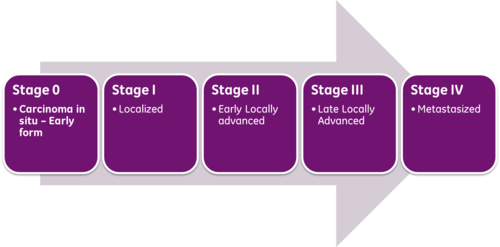
\includegraphics[scale=0.05]{introduction/figures/Cancer_stages.png}
        \caption{Stages of cancer from wikipedia} 
    \end{figure}

        
    Because of this the ability to find, and remove colorectal polyps is excellent for preventing cancer in the GI tract. 
    
    
    \vspace{10px}
    \textbf{colonoscopy/Ontonoscopy}
    In the most common way to look for polyps in the GI tract is to use a medical team, and perform a colonoscopy or Ontonoscopy
Colonoscopy is performed with a camera-stick that is inserted into the GI tract through the patients' anus.\\
    Onoskopy is the same procedure; only the camera is inserted orally. \\
    
    \textbf{Advantages}
      \begin{itemize}
        \item Accuracy: The use of a camera controlled by the doctor gives him/her the opportunity to stop at any anomalies.
        \item Quick results: Since the doctor is doing the procedure the result is given live.
      \end{itemize}

    \vspace{5px}
    \textbf{Disadvantages}
      \begin{itemize}
        \item Expensive: The cost of the doctor and the nurses needed is often high, especially on a routine check.
        \item Invasion of privacy: Getting a Colonoscopy or Onoskopy is a %TODO
      \end{itemize}
    
    \vspace{10px}
    \textbf{MRI}
    MRI (Maggnetic stuff) is the act of taking pictures blabla blabla\\
    MRI (Maggnetic stuff) is the act of taking pictures blabla blabla\\
    MRI (Maggnetic stuff) is the act of taking pictures blabla blabla\\
    %TODO MRI VS CT
    \textbf{Advantages}
      \begin{itemize}
        \item This is why MRI is good %TODO.
        \item This is why MRI is good %TODO.
      \end{itemize}

    \vspace{5px}
    \textbf{Disadvantages}
      \begin{itemize}
        \item This is why MRI is bad %TODO.
        \item This is why MRI is bad %TODO.
      \end{itemize}
    \vspace{10px}
    \textbf{pillcam}
    In the last 3-4 years, there have been testing and development on the pillcam project EIR. Machine learning has, through many of the earlier projects, got the detection rate for the polyps up to x\% %TODO Cite.
    
    \textbf{Advantages}
      \begin{itemize}
        \item This is why pillcam is good %TODO.
        \item This is why pillcam is good %TODO.
      \end{itemize}

    \vspace{5px}
    \textbf{Disadvantages}
      \begin{itemize}
        \item This is why cam is bad %TODO.
        \item This is why pillcam is bad %TODO.
      \end{itemize}
 
    
    
    \vspace{10px}

  \subsection{Simulas contribution to the pillcam project REM}
    Simulas EIR
        

        
    * CAD ACD (computer-aided diagnosis, Automated computer diagnosis)

    \vspace{10px}
    
    


\chapter{Background} \label{cap:background}
\section{Machine Learning}
    Machine learning is a very broad term, but can i short be summarised by:\\
    \vspace{10px}
	
    \textit{ A computer program is said to learn from experience E with respect to 
    some class of tasks T and performance measure P, if its performance at
    tasks in T, as measured by P, improves with the experience E. } 
    \cite{MitchellTomM1997Ml}\\
	
    \vspace{10px}
    Here we have a couple of parameters:\\
    \textbf{E} text about e\\
    \textbf{T} text about t\\
    \textbf{P} text about p\\
	
    From this we see that the goal of machine learning is to improve some performance P with experience.
    \textbf{might here talk about different tasks ML can do?}
    

    \subsection{How machine learning works}   
	\todo{tell that this is loosely based on deeplearningbook, basic machine learning}
	We can start with one of the simplest examples: linear regression. \\
	This is a typical task that is often performed in Machine leaning, though, often the model is often of a polynomial chararcteristics. 
	In linear regression we want to make a model that can predict a value given an input.
	
	\begin{figure}
	    \centering
	    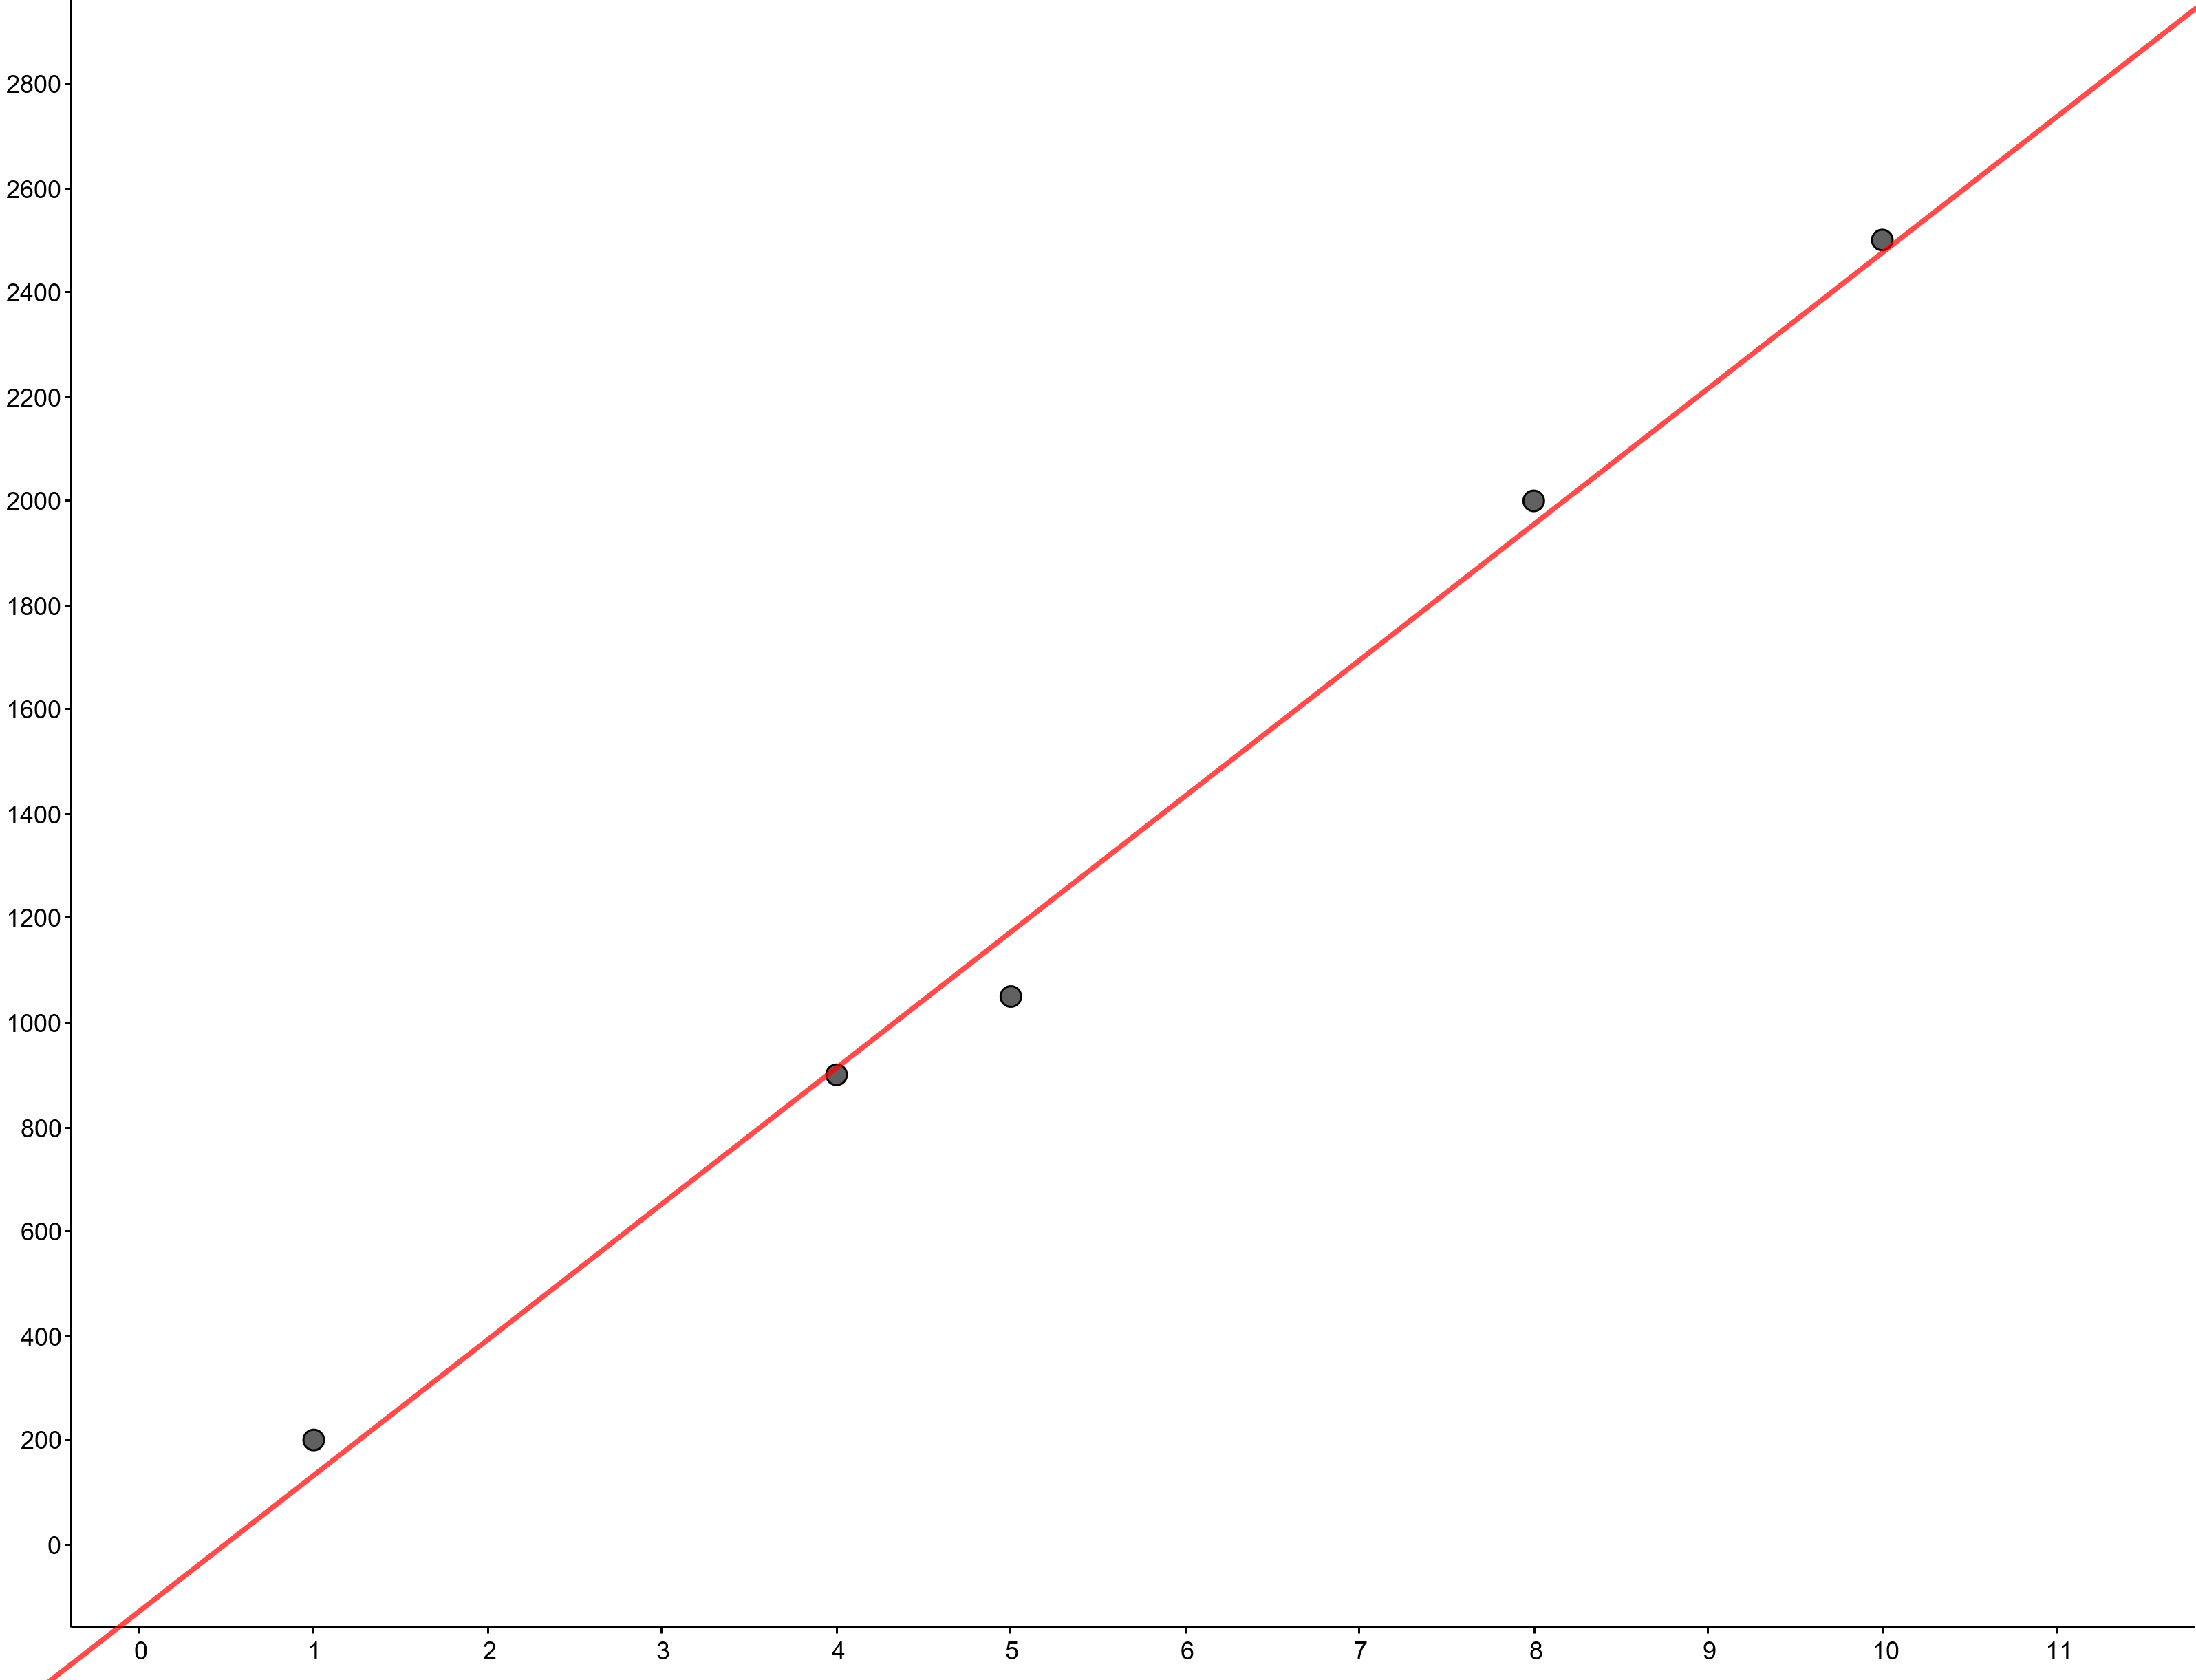
\includegraphics[scale=0.1]{background/figures/linear_regression.png}
	    \caption{Example of linear regression in Geogebra. Here the red line is the best approxmiation of a y value, given an x value.} 
	\end{figure} %credit AK for img
 
	The output, y, from the regression can be calculated with the general formula for a line.
	\begin{equation}
	  y=ax+b\\
	\end{equation}
	Or in the machine learing case:\\
	\begin{equation}
	  y=W^{(1)}x+W^{(2)}\\
	\end{equation}
	Our goal is to find the optimal value for $W^{(1)}$ and $W^{(2)}$ so that the error between the predicted output data and the 
	actual output data is as small as possible.\\
	
	The most prominent way of calculating this error is to use for instance the mean square error betweet the predicet and actual output of the data. 
	\begin{equation}\label{MSE_form}
	 MSE=\frac{1}{2m} \sum_i (\hat{y}-y)_i^2
	\end{equation}
	Where $m$ is the number of samples, $y$ is the real output, and $\hat{y}$ is the prediced output. The 2 in the dinominator is just a constant
	to make derivation of the formula easier.\\
	
	From this we can intuitivly see that the error tends towards 0 when $\hat{y}$=$y$. We can also note, because of the 
	squaring in the formula, that the error is ony based on L2 distance between $\hat{y}$ and $y$.\\
	
	\vspace{10mm}
	Now that we have an error, we need a way to improve it \todo{more about GDEC}
	
	\subsection{Example with gradient decent}
	Now that we have a model with an error function, we can see how we would go on to change the weights ($W^{(1\&2)}$) 
	of our model, to get a better result. 
	
	Lets start with: 
	
	$x=\left[ \begin{array}{c} 1\\ 2\\ 3\\ \end{array} \right]$ 
	and 
	$y=\left[\begin{array}{c} 1.5\\2\\ 2.5\\\end{array}\right]$
	with the weights $W^{(1)}=0$ and $W^{(2)}=0$
	
	We can first calculate the initial loss of the model given a MSE. Using \ref{MSE_form} gives us a loss of:
	\begin{equation}
	   \frac{1}{2*3} (1.5^2+2^2+2.5^2)=2.08
	\end{equation}
	
	
	We will now use gradient decent to estimate
	
	
	
	
	
	\subsubsection{Feed forward}
    
	\subsubsection{Loss and gradient decent }

    
    \subsection{Supervised \& Unsupervised machine learning}
	We often divide machine learning in to two (diffuse) categories: supervised and unsupervised.\\
	\vspace{5px}
	\textbf{Supervised learning:} is the act of training with data that has an answer or a label. The learning algorithm can get supervision while 
	training on the task. An example on a supervised task  is to recognise handwritten numbers, or differentiate between dogs and cats. The task is supervised if the images
	comes with the correct label in the data set. These  examples are typical classification examples, where the task is to identify the right group to classify the data to %TODO more
	A simpler classification assignment is binary classification, where the target is (often) yes or no. Examples for binary classification is if an email is spam or not, is a car Norwegian 
	or International. 
	In the last example the classification changes from binary to multi-class if you sort the cars on every nationality, and not just Norwegian/non-Norwegian.
	  
	Another type of supervised learning is regression. This is the act of prediction given prior data. Examples of regression is everything from prediction of stock prices, to house prices 
	in an area, to\\ %TODO more
	\begin{figure}
	    \centering
	    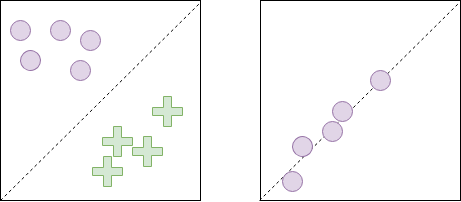
\includegraphics[scale=0.5]{figures/class_vs_reg.png}
	    \caption{Left: Example of binary classification. Right: Example of regression} 
	\end{figure}
  
	\vspace{5px}
	\textbf{Unsupervised learning:} is the act of training without any supervision, on the sense that we do not give the algorithm the answer
	to the training data set. %TODO more 
	 
	Since we do not have categorised data in unsupervised learning, we often %TODO more
	Types of unsupervised learning can for instance be clustering, the act of sorting data based on similarity. An example of this can be if you want to sort plants based on species, or 
	you are detecting anomalies in a dataset.
	Unsupervised learning can be used for PCA %TODO CITE 
	or other dimensionaly reduction methods.\\
	  
	A third method to used unsupervised learning is the adversarial route, where you use machine learning to make similar looking data to the original data set. 
	    
	\begin{figure}
	    \centering
	    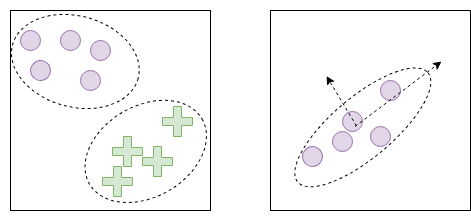
\includegraphics[scale=0.5]{figures/cluster_pca.png}
	    \caption{Left: Example of binary clustering. Right: Example of principal component analysis} 
	\end{figure}

	 
	In the description of supervised vs unsupervised we looked at a specific branch of machine learning: Classification. Classification is, as the name implies, the task of 
	getting data sorted in to groups of similarity. 
	  
	  
	\begin{itemize}
	    \item subsfication
	    \item r to the pillcam projression 
	    \item transcription/translation
	    \item de-noising /finding missing inputs
	\end{itemize}
	  
    \subsection{Types of machine learning (AKA what we can do with ML)}
	There are a number of different machine learning algorithms. %TODO tell that we are going inn to detail here
	\begin{table}[ht]
	    \centering
	    \resizebox{\textwidth}{!}{%
	    \begin{tabular}{|c|c|c|c|c|}
	      \hline
	      \multicolumn{5}{|c|}{Machine Learning}                                                                                 \\ \hline
	      \multicolumn{2}{|c|}{Supervised Learning}   & \multicolumn{2}{c|}{Unsupervised Learning}       & Reinforcement Learning\\ \hline
	      Classification          & Regression        & Clustering           & Dimensionality reduction  & -                     \\ \hline
	      Support vector machines & Linear Regression & K means clustering   & PCA                       & SOMething             \\
	      K nearest neighbours    & Decision trees    & Hidden Markov models &                           &                       \\
	      Neural networks         & Neural networks   & Neural Networks      &                           &                      
	    \end{tabular}%
	    }
	    \caption{Machine leaning types}
	    \label{ML-types}
	  \end{table}
	  
	  %TODO rewrite under.
	  
	  \vspace{5px}
	  \textbf{K nearest neighbours}\\
	  Talk about KNN\\
		
	  \vspace{5px}
	  \textbf{Linear Regression}\\
	  How to regress linearly\\
	  
	  \vspace{5px}
	  \textbf{Support vector machine}\\
	  SVM and 2 class\\
	  
	  \vspace{5px}
	  \textbf{Others?}\\
	  Other important ones to talk about?\\
	
	
	  \vspace{5px}
	  \textbf{Neural networks}\\
	  %TODO har given good results last years
	  %leading in the field
	  %own chapter
	  NN is future\\
	  own chapter\\
	  

	
\section{Neural Networks}
	  
    \subsection{How it works}
	    %TODO talk about backward/forward prop?
	    %
	\begin{figure}[ht!]
	    \centering
	    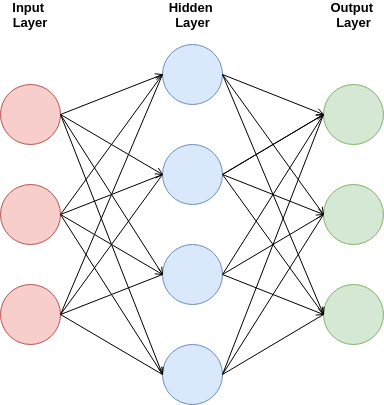
\includegraphics[scale=0.2]{background/figures/neural_network.png}
	    \caption{THIS IMAGE IS SHAME(LESS)LY taken from the internetz, draw own so the lawyers don't get you!}
	\end{figure}
	TEXT ABOUT NEURAL NETWORKS\\
	TEXT ABOUT NEURAL NETWORKS\\
	TEXT ABOUT NEURAL NETWORKS\\
	TEXT ABOUT NEURAL NETWORKS\\

	
	TEXT ABOUT FEED FORWARD\\
	TEXT ABOUT FEED FORWARD\\
	TEXT ABOUT FEED FORWARD\\
	TEXT ABOUT FEED FORWARD\\

	TEXT ABOUT BACKPROP\\
	TEXT ABOUT BACKPROP\\
	TEXT ABOUT BACKPROP\\
	TEXT ABOUT BACKPROP\\
	
    \subsection{Convolutional neural networks}
	\begin{figure}[ht!]
	    \centering
	    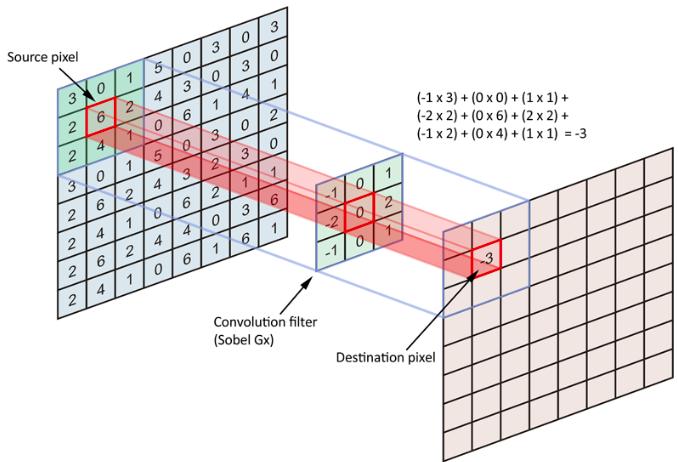
\includegraphics[scale=0.2]{background/figures/conv_neural_network.png}
	    \caption{THIS IMAGE IS SHAME(LESS)LY taken from the internetz, draw own so the lawyers don't get you!}
	\end{figure}
    
    \subsection{Advaserial neural networks}
  	  	\paragraph{This is explaining GANS, put me in the right place} %%TODO CITE: http://www.deeplearningbook.org/contents/generative_models.html and Goodfellow at al. 2014
	  Now that we have looked at autoencoders we can take it a step further. 
	  generative advaserial models can be used as a generator of new data, and can have som reseblance to autoencoders \ref{Explaining_autoencoders}, especially variational autoencoders %TODO cite VAE, ref VAE
	  
	  The difference lies in that advaserial networks is based on game theoretic scenarios in which a generator network is compeating agenst an advasery. 
	  The generator produces samples $x=g(z;\theta^{(g)})$, where $g$ is the network given the weights $\theta$. Then the discriminator network predicts if a sample is drawn from the dataset or from the generator.
	  More spessific, it gives a probably given by $d(x;\theta^{(d)})$ , and determins if $x$ is from the generator or the data-set. 
	  Since we have two networks compeating agenst each other we can look at this as a Zero-sum game with the generators payoff is determined by $v(\theta^{(g)},\theta^{(d)})$, and the discriminators payoff is determined 
	  by $-v(\theta^{(g)},\theta^{(d)})$.
	  \textit{$v$ is here a function that is determined by both the sucsess rate of the discriminator and the generator, the most common used is}
	  \begin{equation}
	  v(\theta^{(g)},\theta^{(d)}) \; = \; \mathds{E}_{x\sim p_{data}}\log{d(x)} + \mathds{E}_{x\sim p_{model}}\log{(1 - d(x))} %TODO: CITE First gan paper on formula
	  \end{equation}
	  as derived from Goodfellow et al. %TODO cite 
	  
	  Lets look at a gan in detail. \\
	  \begin{figure}[ht!]
	    \centering
	    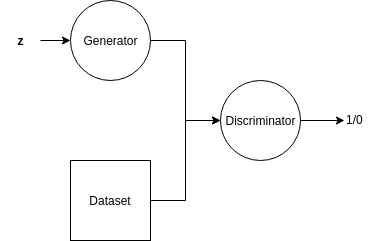
\includegraphics[scale=0.5]{background/figures/simpleGAN.png}
	    \caption{The idea behind a GAN. Here the generator saples from a random (Gaussian) distribution and generates samples that the discriminator classifies as real or fake}
	\end{figure}
	
	 %TODO MORE
    \subsubsection{UCNN?}	
    \subsection{Recurrent neural networks}
      \subsubsection{LSTM}
	
	
\section{Models we need to explain at this point (find better tittle)}
    \subsection{Autoencoders}\label{Explaining_autoencoders}
	  %%TODO CITE: http://www.deeplearningbook.org/contents/autoencoders.html
	  As we recall from earlier, an autoencoder is a type of neural network that tries to output a recreation of the output.\todo{we are not recalling} \\ 
	  
	  We can do this by having an encoder, $h=f(x)$, connected to a decoder, $r=g(h)$. 
	  An autoencoder has the job to set $g(f(x))=x$ over the whole input, but in most cases this is not a practical program. We often gives the autoencoder the restriction
	  that it has to map the input through a latent space that has a smaller dimension than the input dataset.\\
	  This is called an undercomplete autoencoder.\\
	  \vspace{10px}
	  \begin{figure}[ht!]
	    \centering
	    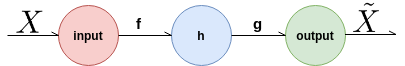
\includegraphics[scale=0.5]{background/figures/SimpleAE.png}
	    \caption{The general structure of an autoencoder, mapping $\textbf{x}$ through $\textbf{h}$ to an output $\textbf{r}$.}
	  \end{figure}
	  
	  As with supervised classifiers we can use gradient decent to optimize the model. This is because we are trying to recreate the input $\textbf{x}$ from out output $\widetilde{\textbf{x}}$\\
	  
	  This can simply be done by minimizeing the loss function\\
	  \begin{equation}
	    L(\textbf{x},g(f(\textbf{x})))
	  \end{equation}
	  with for instance MSE with gradient decent. \todo{explain MSE, and general loss on an ealier time}\\
	  
	  Now we can transfer this to a more relevant example by making an image as input and use convolutions to reduce the dimensionality in the encoder and increase the dimentionality in the encoder.
	  \vspace{10px}
	  \begin{figure}[ht!]
	    \centering
	    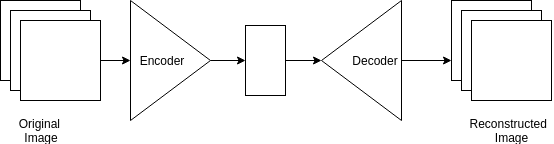
\includegraphics[scale=0.5]{background/figures/CAE.png}
	    \caption{Convolutional autoencoder with an RGB image as input, and the reconstructed image as output.}
	  \end{figure}
	
    
    
    \subsection{Contextencoders}
	Inpainting can also be done with advaserial models, and using a network trained to do the task of inpainting can be a lot more powerful than using just an autoencoder\todo{ref} or the naive methods\todo{ref}.
	A contextencoder is building on the advaserial principle by using a generator/discriminator pair to fill in masked areas in an image. 
	
	The concept behind a Contextencoder is to take the whole image as input to an encoder/decoder pair and \todo{finish}
    
    
    \subsection{CC-GANS}
      HERE IS TEXT ABOUT CCGANS
      HERE IS TEXT ABOUT CCGANS
      HERE IS TEXT ABOUT CCGANS
      HERE IS TEXT ABOUT CCGANS
      HERE IS TEXT ABOUT CCGANS
      HERE IS TEXT ABOUT CCGANS
      HERE IS TEXT ABOUT CCGANS
      HERE IS TEXT ABOUT CCGANS
      HERE IS TEXT ABOUT CCGANS
      HERE IS TEXT ABOUT CCGANS
      HERE IS TEXT ABOUT CCGANS
      HERE IS TEXT ABOUT CCGANS
      HERE IS TEXT ABOUT CCGANS
      HERE IS TEXT ABOUT CCGANS
      HERE IS TEXT ABOUT CCGANS
      HERE IS TEXT ABOUT CCGANS
      HERE IS TEXT ABOUT CCGANS
      HERE IS TEXT ABOUT CCGANS
      HERE IS TEXT ABOUT CCGANS
      HERE IS TEXT ABOUT CCGANS
      HERE IS TEXT ABOUT CCGANS
      HERE IS TEXT ABOUT CCGANS
      HERE IS TEXT ABOUT CCGANS
      HERE IS TEXT ABOUT CCGANS
      HERE IS TEXT ABOUT CCGANS
    
    
    \subsection{Pixel CNN}
      HERE is text about pccn
      HERE is text about pccn
      HERE is text about pccn
      HERE is text about pccn
      HERE is text about pccn
      HERE is text about pccn
      HERE is text about pccn
      HERE is text about pccn
      HERE is text about pccn
      HERE is text about pccn
      HERE is text about pccn
      HERE is text about pccn
      HERE is text about pccn
      HERE is text about pccn
      HERE is text about pccn
      HERE is text about pccn
      HERE is text about pccn
      HERE is text about pccn
      HERE is text about pccn
      HERE is text about pccn
      HERE is text about pccn
      HERE is text about pccn
    


\section{Cancer and polyps}
	  \subsection{What is the GI tract REM}
	  \subsection{How does polyps form REM}
	  \subsection{What we are looking for REM}
	  Different types of disorders.
	  %TODO image of polyp
	  Polyp is harmless, but if left untreated it can become cancerous
	  %TODO tell the risk
	  Pictures is from the pillcam project, kvasir dataset.
	  \subsection{images from pillcam, and what we are looking at/for REM}
	  %TODO More pictures of polyps, and other anomalies
	  

	  
	  

	    
	  
\section{Explain how the ML-methods can be used with the polyps}
	When you work with machine learning a lot of the job is to make the data as clear as possible. \\
	Imagine that you want to do something simple as reading an analogue clock. The \"straight forward\" way to do it is to  
	make a convolutional neural network to look at the dials. This will require a much more complex network compared to if you could convert the angle of the dials
	to degrees and have that as an input to your model.

	\begin{figure}[ht]
	  \centering
	  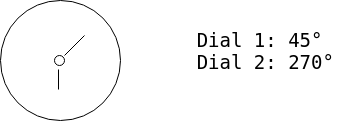
\includegraphics[scale=0.5]{methods/figures/Clock.png}
	  \caption{A clock needs a more complex network compared to just the degrees}
	\end{figure}
	%TODO FIND ORIGinal source
	The trick is often to make the data as refined as possible. 
	Further some of the techniques used is described.
	
	\todo{Here i need to talk about how preproccesing might help the problem, and make this a springboad in to the next section: the problem at hand}
	
	
	\todo{adress the problem with lack of data, and talk about how machine learning can help, machine learning.}
	  
	  
\section{The problem at hand}
	  Now that we have the definition of machine learning and the current task, we can focus on the task at hand; finding polyps. In an ideal world\footnote{Ideal as in the only disease we could get in  the GI tract was cancer originating
	  from polyps which looked exactly the same} we have a
	  Classification problem with only two classes: Non-polyp and polyp. 
	  
	  \begin{itemize}
	    \item SVM 
	    \item CNN 
	    \item random forests
	    \item knn
	  \end{itemize}
	  
	
	\section{In painting}
  We have discussed the importance of good input data, and the potential benefits to resource usage and ease of making a good model.
  So a priority when it comes to image classification is to have data without anomalies and other areas that can be interpreted as a feature for the classifier. 
  In a machine learning perspective, the data is best if it has the same structure, and is %TODO similar enough.
  In painting is the process of reconstructing lost or deteriorated parts of images and videos. %TODO CITE https://en.wikipedia.org/wiki/Inpainting
  

  From prior papers on polyp detection in the GI tract %TODO CITE!!!
  we have clear results that the black corners, and the green squares trigger a big activation %TODO WRITE BETTER
  when it comes to classifying images. 
  From %TODO CITE, find out who
  's paper, we can see that the activation map on a regular image gives very high result on, in addition to the polyp, the corners and the green sqare. 
  \begin{figure}[ht]
    \centering
    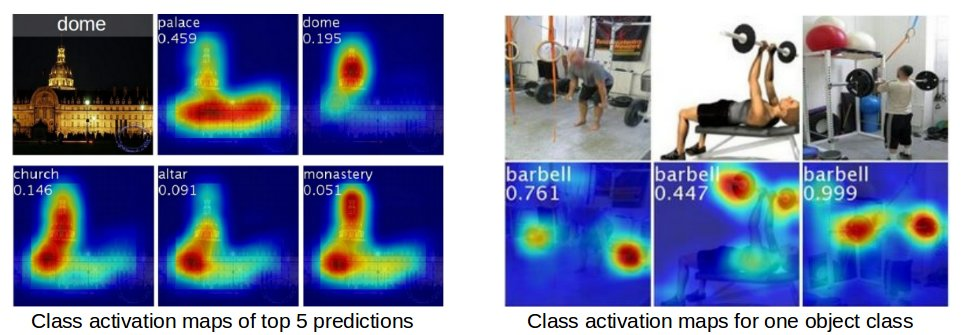
\includegraphics[scale=0.5]{background/figures/placeholder.jpeg}
    \caption{Using X's activation map we can see that the edges triggers unwanted activations}
  \end{figure}
  
  In addition to sqares and edges, we also have the problem that parts of the image is over saturated at points where the light from the led is reflected directly back to the camera.
  Another problem is when the camera captures images that are too close to the wall. Both of these scenarios creates patches where the saturation is maximum. 
   \begin{figure}[ht]
    \centering
    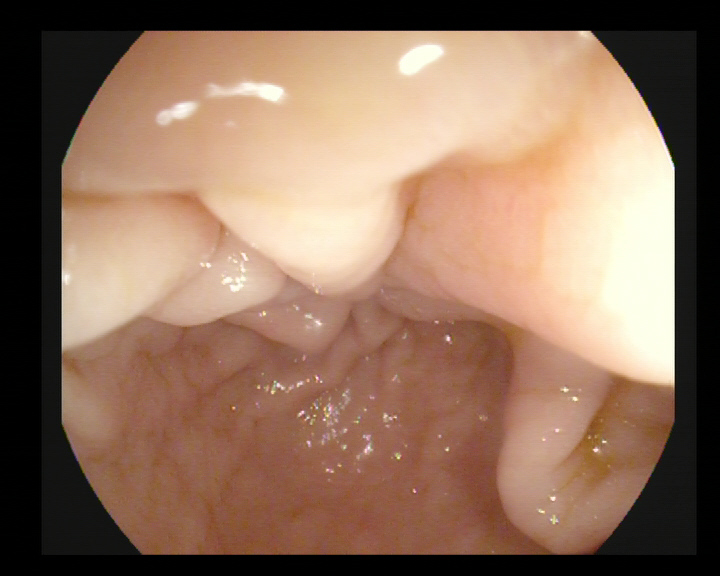
\includegraphics[scale=0.5]{background/figures/reflection.jpg}
    \caption{we have two different types of saturation: the reflected area in the top part of the image, and the right side of the image.}
  \end{figure}
  in an ideal scenario the image would have no pixel values at max, and as little frame as possible. 
  We therefor want to make a tool that can help us with this.
  \subsection{Naive methods for In painting}
    Inpainting is not a new area of research, as it has been around since %TODO CITE
    Because of this there are many naive methods that gives good inpaintings. 
	
    \subsubsection{Textured syntesys based on image inpainting}
    \subsubsection{MOARE}
    \subsubsection{MOARE}
   \subsection{Naive methods for borderfinding}

%
% THIS SECTION MUST BE MOVED/FIXED
%
\section{Naive Methods REM}
	  Now that we have an idea of what we are looking for we can first turn to some more naive methods for detecting anomalies, and for enhancing the images.\\
	  The field of image processing has been researched since\\ %TODO WHEN
	  
	  Using some of the classic methods in image processing we can see if\\ %TODO
	  
	  We often describe the method in to two groups of information: First and Second order statistics.\\
	  \textbf{First order:} First order statistics does not take in to account the relative positioning of the pixels in the image, and because of this, gives much less
	  information than the second order statistics.\\
	  Example of First order statistics is often what information we can get out of a histogram. This can be scewness, variance, and mean value.\\
	  
	  \vspace{10px}
	  
	  \textbf{Second order:} Second order statistics takes in to account the relative positioning of the pixels in the image. We can calculate the GLCM matrix and get a much more detailed 
	  view of the image. \\
	  
	  
	  
	  \subsection{GLCM}
	    A GLCM (Grey-level co-occurrence matrix) is a matrix that is used when examining the spatial relationship of pixels in a texture. 
	    The calculation of a GLCM gives us how often pairs of pixels with spesific values and a specified spatial relationship occur at a given place in an image. %TODO CITE
	  
	    \subsubsection{Algorithm}
	      For simplicity we use only greyscale in this example:
	      \begin{figure}[ht]
		\centering
		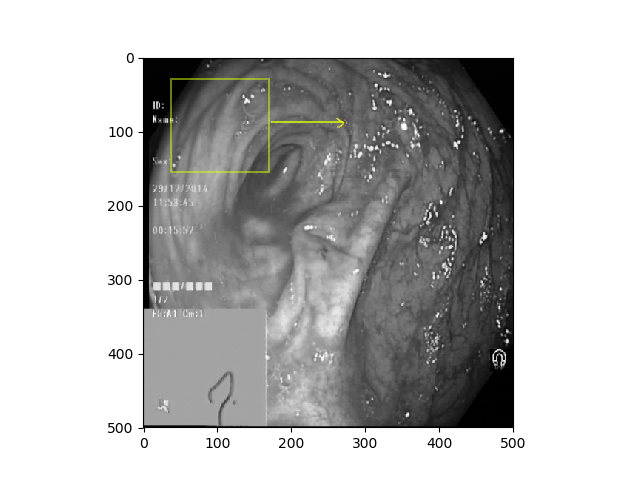
\includegraphics[scale=0.5]{figures/sliding_window_box.png}
		\caption{GLCM capturing features}
	      \end{figure}
	      The algorithm starts by running a sliding window over the image, often with a stride, and for each stops calculates the spatial relationship between each pixel specified.
	      The result can be something like this figure %TODO link to figure
	      where we can read out the most likely neighbouring pixel.
	       \begin{figure}[ht]
		\centering
		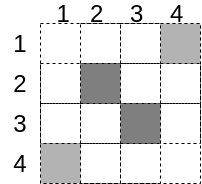
\includegraphics[scale=0.5]{figures/Simple_GLCM.png}
		\caption{GLCM Matrix}
	      \end{figure}
	      The darker colours on in the matrix is indicating that we often have a jump between, for instance pixel-value of 1 and a pixel-value of 4, but no from 1 to 1.\\
	      With this information we can get a naive pattern-recogniser. 
	    \subsubsection{Other uses}
	      Besides for the pattern recognition we can use the GLCM to get the information on:
	      \begin{itemize}
	       \item \textbf{Contrast} is the difference in luminance or colour in the picture. We would expect low contrast in the “background” and higher contrast around edges and irregular objects.
	       \item \textbf{Homogeneity} is how similar a local area is to itself
	       \item \textbf{Variance} $\sigma^2$ , is directly a measure of ”roughness”
	       \item \textbf{Mean} value of a GLCM can give us areas with higer or lower pixel values. Good way to find polyps if they are lighter than the tissue around.
	       \item \textbf{Entropy}
	       \item \textbf{Energy}
	      \end{itemize}


	  
	  \subsection{Edge detection}
	    Using Edge detection in is another viable way to look for polyps. 
	    \begin{figure}[ht]
	      \centering
	      \begin{minipage}[b]{0.45\textwidth}
		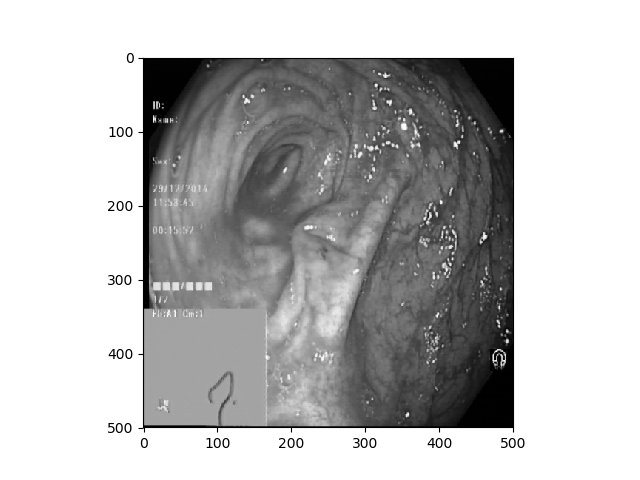
\includegraphics[width=\textwidth]{figures/sliding_window.png}
		\caption{Original image}
	      \end{minipage}
	      \hfill
	      \begin{minipage}[b]{0.45\textwidth}
		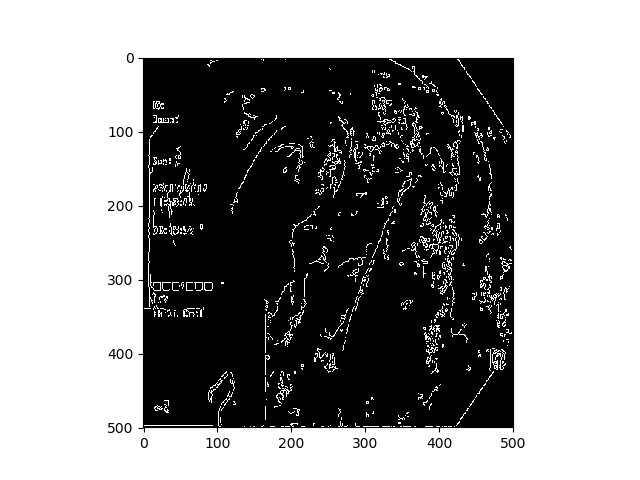
\includegraphics[width=\textwidth]{figures/Canny.png}
		\caption{Edges of the picture}
	      \end{minipage}
	    \end{figure}
	    \subsubsection{Algorithm}
	      For each pixel look at the neighbouring pixel, if \\
	      
	      \begin{centering} 
		$ abs(p_a - p_b)>tresh $\\ 
	      \end{centering}
	      
	      then mark pixel as an edge pixel. \\
	      
	  \subsection{Hough Transforms}
	    Using for instance Canny edge detection %TODO CITE
	    we can get a better view of where the potential border of the polyp/anomaly is. (As shown in %TODO FIG CITE)
	    
	    A hough transform can i theory have many/any shape(s), and together with edge detection, we might find some of the polyps this way.
	    
    
    
    
    
    
	
    As we can see from this, there are a lot of old methods that can give approximations. We can also conclude that none of these methods are perfect.
    We will therefore look at methods that takes learning in to use.
\section{Using machine learning for inpainting}
    \subsection{AE}
    \subsection{CE}
    \subsection{CCGAN}
    \subsection{PCNN}
    As discussed earlier, machine learning is using prior experiences to make decisions given the problem at hand. 
    It is also worth mentioning that we do not need labeled data, since we are in a way looking at a global average of every image both with, and without polyps. We are therefor incentiviced to use an 
    Unsupervised approach.
    Since machine learning is learning from a training set, it is important that the training set contains as little as possible of the features we want to remove. \\
    
    Because of this the first thing we need to do if we are going to mask out corners and sqares, is to limit the training set to only contain cropped, non-sqare images. 
 
    \begin{figure}[ht]
      \centering
      \begin{minipage}[b]{0.45\textwidth}
	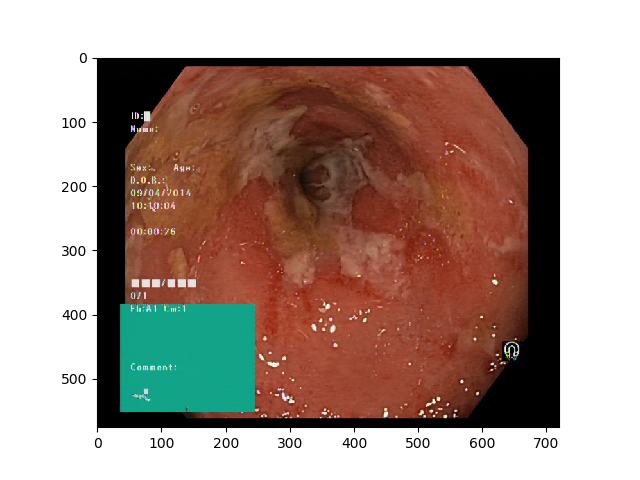
\includegraphics[width=\textwidth]{background/figures/uncropped_img.png}
	\caption{Original image with black padding}
      \end{minipage}
      \hfill
      \begin{minipage}[b]{0.45\textwidth}
	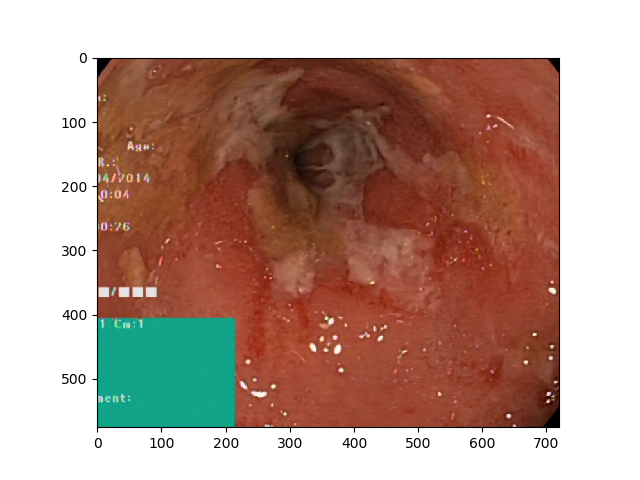
\includegraphics[width=\textwidth]{background/figures/cropped_8percent_img.png}
	\caption{Black edges cropped away + 8\% zoom}
      \end{minipage}
      \caption{Here we have an example on how we would make an image better to train on. This is not representative of the training, since we only use images without the green square under training}
    \end{figure}
    
    Now that we have better images to train our data with, we need the correct algorithm.
    We have already seen unsupervised learning aproaches in chapter %TODO ref 
    \newpage
    \subsubsection{Algorithm}
      \todo{Hvordan skal jeg gaa frem nar det kommer til aa presantere disse? skal jeg bare si hvilke metoder jeg har testet?}
      Text about presenting UML, and stuff.
  
	\newpage
	As we recall from earlier, an autoencoder is a type of neural network that tries to output a recreation of the output.\\%TODO: REF the part about autoencoders 
	We can use this for inpainting by setting the algorithm to train on images with areas cropped away.
	There are a couple of different way we can train an autoencoder to do this.\\
	
	%\todo{should i talk about the different ways or present the best?}
	
	
	\vspace{10px}
	\textbf{Denoising Autoencoder with MSE loss:}\label{par:Denoising_Autoencoder_with_MSE_loss}\\
	The simplest way to train the autoencoder is to first take the trainingset $\mathds{X}$ and make an augmented copy $\widetilde{\textbf{x}}^{(i)}$ for 
	every data point in $\textbf{x}_{\sim \mathds{X}}^{(i)}$. \\
	\textit{Here $\widetilde{\textbf{x}}$ is a copy of x with random areas masked.}\\
	
	Now we minimize the loss function\\	
	  \begin{equation}
	    L(\textbf{x},g(f(\widetilde{\textbf{x}})))
	  \end{equation}
	over the whole image.\\
	\vspace{20px}
	
	With this approach the autoencoder learns to fill in the blank spots with plausible data, without changing the rest of the image. 
	\todo{this will probably work best if the autoencoder is not undercomplete, perhaps talk about this}
	One problem by this approach is that we do not want the rest of the image to change for obvious reasons, and the alogrithm as it is here has the flaw that it will change all the pixels in the image, at 
	least to a minor degree. \\
	
	This can be somewhat fixed by only taking the augmented parts, and pasting the directly in to the image. This will leave most of the original image, except for the parts that was cropped randomly.\\
	
	\vspace{10px}
	\textbf{Denoising Autoencoder with \todo{clever tittle}:}\\
	If we take what we learned from \ref{par:Denoising_Autoencoder_with_MSE_loss}, we can make a more optimal autoencoder:
	Rather than taking a loss like 	
	\begin{equation}
	  L(\textbf{x},g(f(\widetilde{\textbf{x}})))
	\end{equation}
	over the whole image, we can rather just focus on the parts that matters, namely the cropped areas.\\
	
	If we add the cropped image to the output from the autoencoder to make an image image, we can use this new image to train out loss.
	For most of the image, the loss will be zero, since the only part that is changed is the cropped area. 
	We can also make a new loss that is more optimal for the task at hand. 
	\begin{equation}
	  MSE_{crop}\:=\: \frac{1}{n}
	  \begin{cases}
	      \begin{array}{lcl}
	      (\widetilde{\textbf{x}}-\textbf{x}) \; if \; \widetilde{\textbf{x}} \: \in \: \textbf{x}_{crop} \\
	      0 \; else
	      \end{array}
	  \end{cases}
	\end{equation}
	Where $\textbf{x}_{crop}$ is the area that was cropped away from the original image and $n$ is the number of pixels in that area.\\
	With this modified MSE we are assured that only the pixels in the cropped area is changed with gradient decent, and we save a lot of computation as an added bonus.
	
	
	\todo{token to not train}
	\begin{figure}[ht!]
	    \centering
	    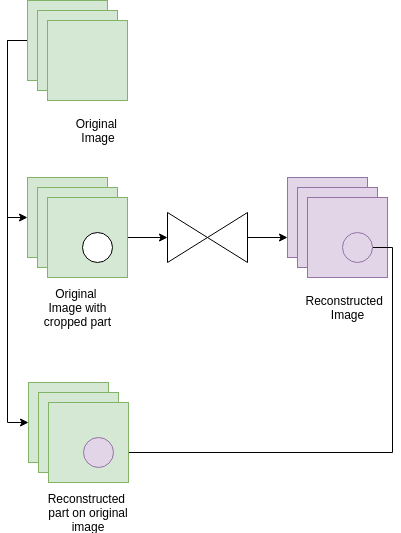
\includegraphics[scale=0.5]{background/figures/AE_for_inpainting.png}
	    \caption{Final result of the autoencoder used in the testing}
	\end{figure}
	
	
	
	
	
      \subsubsection{Explaining GANs, this will be moved}
      
	
      \subsubsection{Contextencoder}
	Inpainting can also be done with advaserial models, and using a network trained to do the task of inpainting can be a lot more powerful than using just an autoencoder\todo{ref} or the naive methods\todo{ref}.
	A contextencoder is building on the advaserial principle by using a generator/discriminator pair to fill in masked areas in an image. 
	
	The concept behind a Contextencoder is to take the whole image as input to an encoder/decoder pair and \todo{finish}
	
	
	
      \subsubsection{CCgan}
      \subsubsection{PixelCNN}
      
  
 



%\part{The project}
\chapter{Methodology}\label{cap:methodology}
With our background in both medical background and machine learning, we can now look at how we want to solve the problems associated with setting up a system for medical diagnosis.  
We will first get a birds-eye view of the objective of this thesis, looking at the hypothesises behind this thesis, and take a look into how we can test the proposed hypothesises. We look at the proposed program setup to test the hypothesises both for classification and generation.
Then we look at the language and packages suitable for this project. We go in-depth into the reasoning behind why we chose the tools and packages that became the foundation of the programs. 

%Then we look at the setup of the complete program. Here we will go in-depth into both the different preprocessing algorithms, and take a look at the transfer learning network used during classifying.

\section{ Bird's eye view (Chapter possibly removed when written)}
\label{cha:BEW}
In the summary of the background chapter, we looked at two articles published by Pogorelov et al. and Hicks et al. where they discussed the effect of overfitting and the consequences of dataset-specific artefacts.
To help solve these predicaments look back at the two hypothesises presented in section~\ref{cha:problemstatement}:

\vspace{2px}
Hypothesis~\ref{hyp:a} stated that sparse information in the images made it harder to classify the images correctly. Figure \ref{fig:Saliencymasks} from Hicks's paper shows the case where the black areas with sparse information affect the classification. As we can see, the black areas trigger as a ``positive'' in some om the saliency maps. We can interpret this as the network learning features not useful for the classification. 
Our quest is to check the validity of this hypothesis. We propose to test the classification of images with and without areas with sparse information.


\vspace{5px}
Hypothesis~\ref{hyp:b} stated that dataset specific artefacts create false positives and negatives. This error is clearly shown in \ref{fig:sal2}, where the classification is affected by the green square in the image. 
As long as the classification is affected by dataset specific artefacts, the ability to adapt the dataset to new use cases might suffer.  


\begin{figure}
     \centering
     \begin{subfigure}[t]{0.3\textwidth}
         \centering
         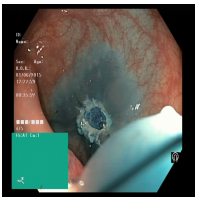
\includegraphics[width=\textwidth]{methodology/figures/sal1.png}
         \caption{Original image that are classified}
         \label{fig:sal1}
     \end{subfigure}
     \hfill
     \begin{subfigure}[t]{0.3\textwidth}
         \centering
         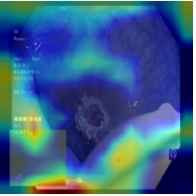
\includegraphics[width=\textwidth]{methodology/figures/sal2.png}
         \caption{Heatmap of the decision}
         \label{fig:sal2}
     \end{subfigure}     
     \hfill
     \begin{subfigure}[t]{0.3\textwidth}
         \centering
         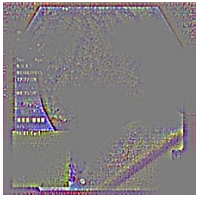
\includegraphics[width=\textwidth]{methodology/figures/sal3.png}
         \caption{Heatmap of the decision}
         \label{fig:sal3}
     \end{subfigure}
     \caption{Saliency maps}
     \label{fig:Saliencymasks}
\end{figure}

\begin{figure}
     \centering
     \begin{subfigure}[t]{0.3\textwidth}
         \centering
         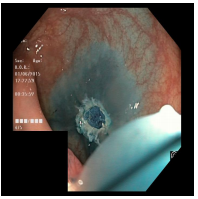
\includegraphics[width=\textwidth]{methodology/figures/sal4.png}
         \caption{Original image that are classified}
         \label{fig:sal4}
     \end{subfigure}
     \hfill
     \begin{subfigure}[t]{0.3\textwidth}
         \centering
         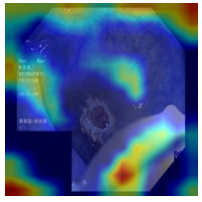
\includegraphics[width=\textwidth]{methodology/figures/sal5.png}
         \caption{Heatmap of the decision}
         \label{fig:sal5}
     \end{subfigure}     
     \hfill
     \begin{subfigure}[t]{0.3\textwidth}
         \centering
         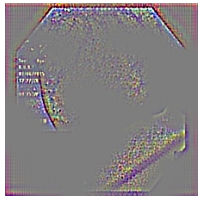
\includegraphics[width=\textwidth]{methodology/figures/sal7.png}
         \caption{Heatmap of the decision}
         \label{fig:sal7}
     \end{subfigure}
     \caption{Saliency maps}
     \label{fig:Saliencymasks2}
\end{figure}



We note that \ref{hyp:a} concerns both training and testing on the same dataset, while \ref{hyp:b} is more concerned about the generalisability of the model, and hence the goal is to use different datasets for training and testing, as well as testing at the training set. 



%As described in the background chapter, we will use convolutional neural %networks to augment and classify the datasets. We will first talk about the programming language in question followed by a rundown of the libraries and their dependencies.
%We end this chapter by looking at the programs used for inpainting and classification.
\todo{talk more about the differnt images in relation to steven.}


To test the two hypotheses, we first need new datasets to compare against a base case. In addition to the dataset with sparse information and dataset-specific artefacts, we need similar looking datasets without these unwanted features. In an ideal scenario, we would have the same dataset without the features added post-capture. 

When it comes to real machine learning gathering (labelled) data for the training is often a challenging task. In this thesis, we have decided to focus our attention in to modifying existing data instead of finding new data. 

We propose to use unsupervised machine learning to inpaint the areas with dataset specific artefacts as well as sparse areas. We then propose a transfer learning network to classify the newly created images. 

\todo{More here i feel}

\FloatBarrier
\section{Design of the inpainting algorithms}

We first want to set up a platform where every dataset is made with the same parameters, except for the dataset-specific parameters that define the dataset. 
When generating the datasets, we use the Kvasir dataset~\cite{Pogorelov:2017:KMI:3083187.3083212} as the training set, as Hicks et al. did in their paper on removing dataset specific artefacts~\cite{25956}. In addition, we use datasets without the artefacts for testing.
This selection of image source was made intentionally to have a fundamentally different test and training set, and the more differences between testing and training set the more of an indication of generalisation. 

Figure \ref{fig:KvasirAnomaliesFIX} shows two different image types from the Kvasir dataset. 
Figure \ref{fig:LargeLeftBlack} shows an image of esophagitis. This image shows one of the main problems with the Kvasir dataset when it comes to artefacts. In addition to the cut corners, we have an extra wide area to the left of the image containing non-relevant information like name, sex, and other comments. This area gives us ample opportunity to test hypothesis \ref{hyp:a}, given that the image contains a large amount of sparse information that we want to remove to see the effect on classification. We believe that if we can change images like Figure \ref{fig:LargeLeftBlack} into images like in Figure \ref{fig:LargeLeftBlackFIX} we will see an improvement in classification when testing and training on the same images.

Figure \ref{fig:GreenSquareOccluding} shows another problem with datasets like Kvasir.  Here we have a green square in the bottom left corner that occludes parts of the image and the same type of text displaying name age and other non-relevant information. We recall from section \ref{cha:BEW} that information like this can give the classifier false positives, and subsequently provide us with a lower classification score. 
We believe that if we can change images like Figure \ref{fig:GreenSquareOccluding} into images like in Figure \ref{fig:GreenSquareOccludingFIX} we will see an improvement in classification when testing and training on different datasets.


\begin{figure}
     \centering
     \begin{subfigure}[b]{0.4\textwidth}
         \centering
         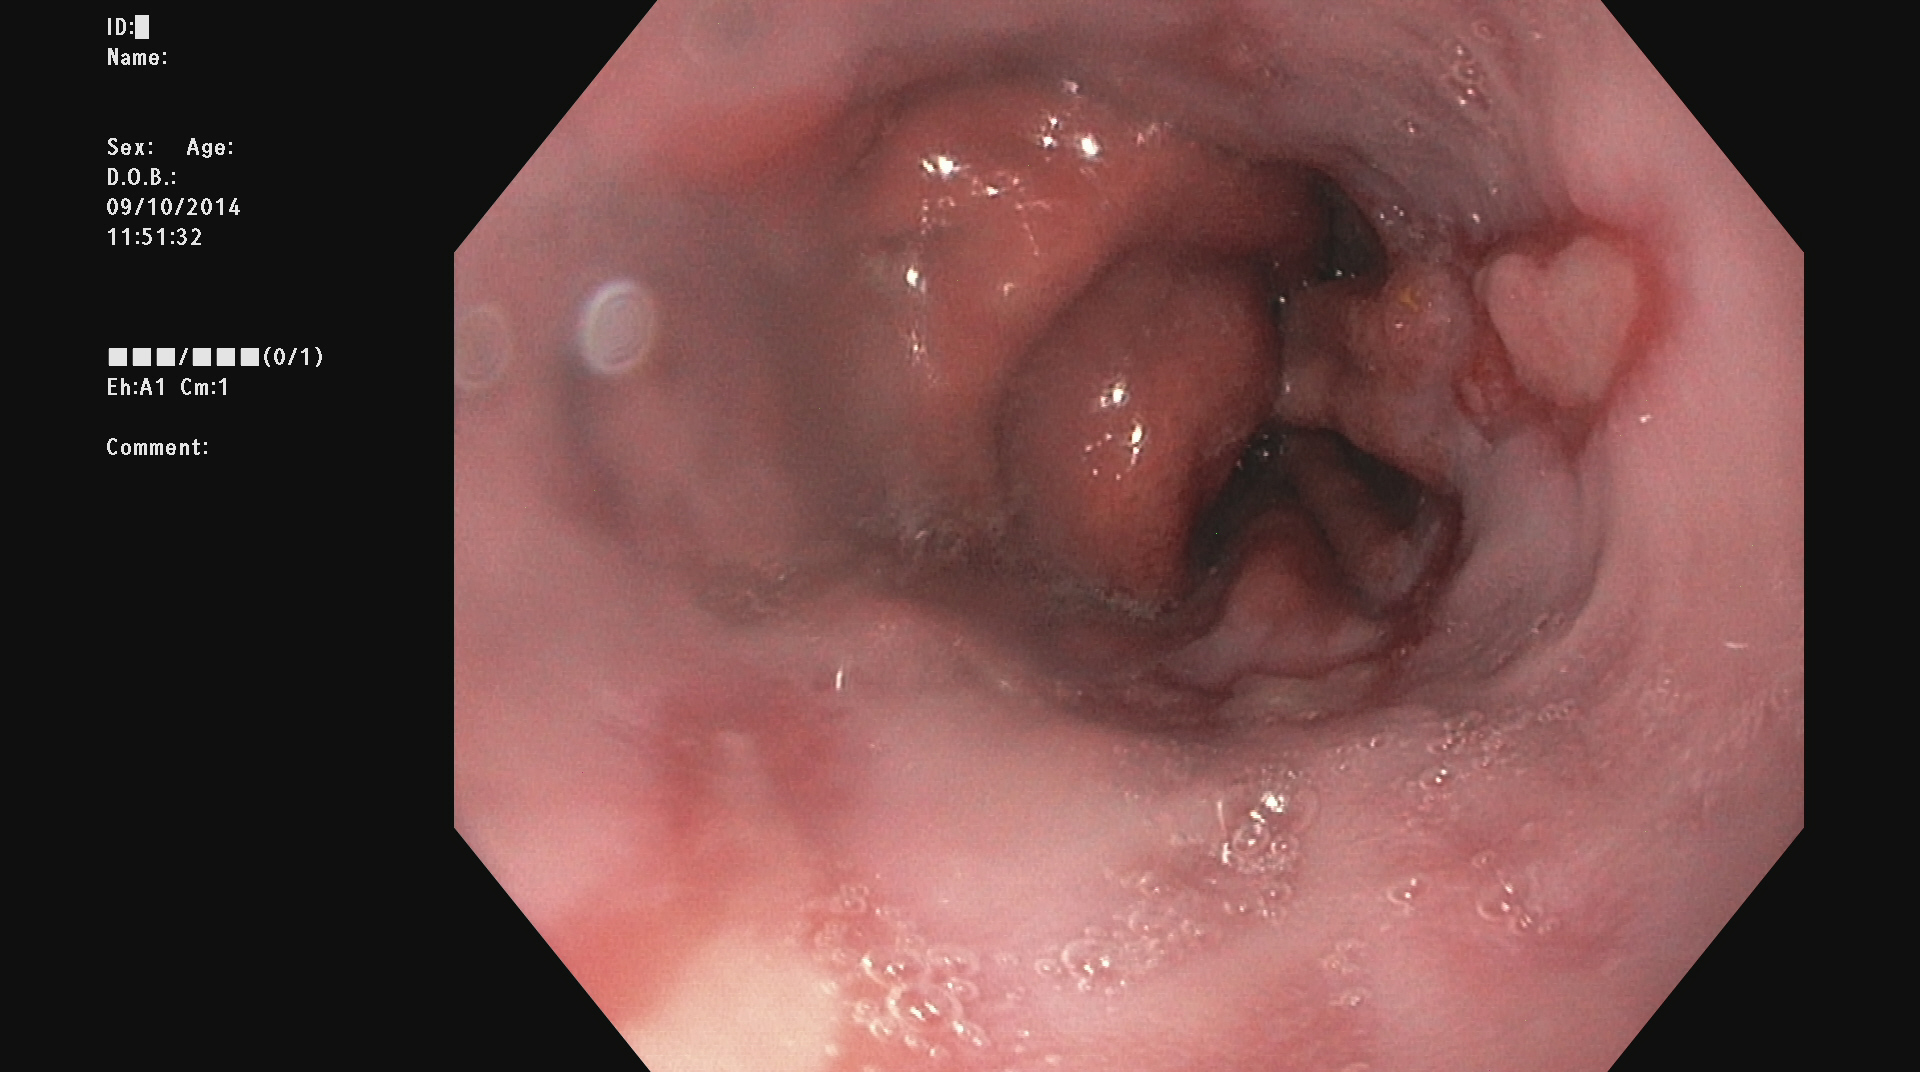
\includegraphics[height=5cm,width=\textwidth]{experiments/figures/leftframe.jpg}
         \caption{Example of an image with a large area without relevant medical information}
         \label{fig:LargeLeftBlack}
     \end{subfigure}
     \hfill
     \begin{subfigure}[b]{0.4\textwidth}
         \centering
         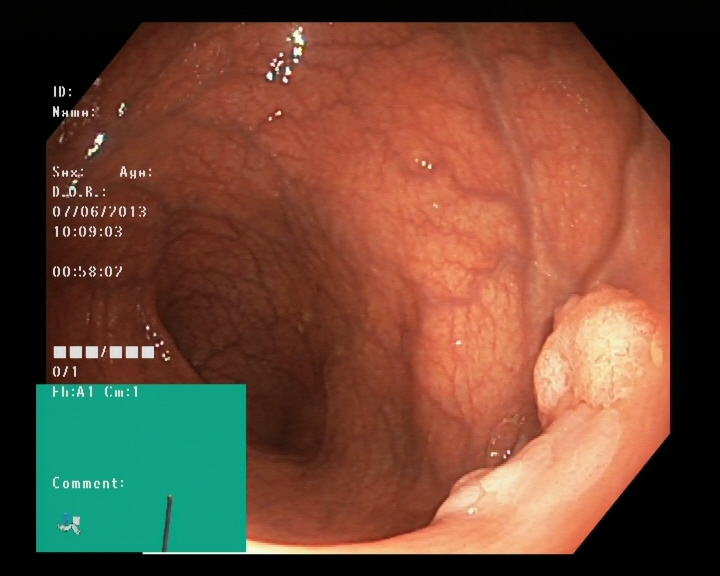
\includegraphics[height=6cm,width=\textwidth]{experiments/figures/greenframe.jpg}
         \caption{Example of an image with green square occluding the parts of the GI tract}
         \label{fig:GreenSquareOccluding}
     \end{subfigure}     
     \hfill
     \begin{subfigure}[t]{0.4\textwidth}
         \centering
         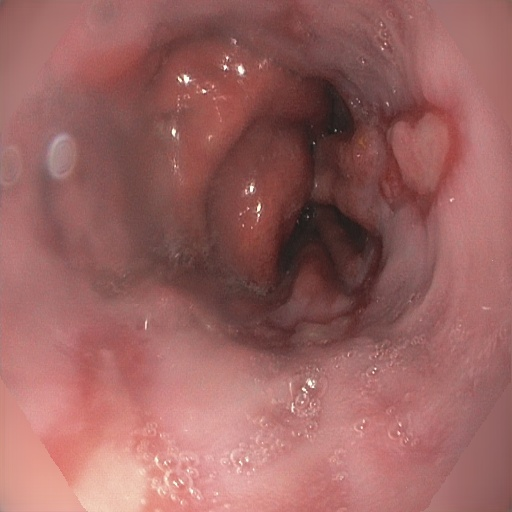
\includegraphics[width=\textwidth]{experiments/figures/noleftframe.jpg}
         \caption{The same image as in Figure \ref{fig:LargeLeftBlack} with the non-relevant information removed}
         \label{fig:LargeLeftBlackFIX}
     \end{subfigure}
     \hfill
     \begin{subfigure}[t]{0.4\textwidth}
         \centering
         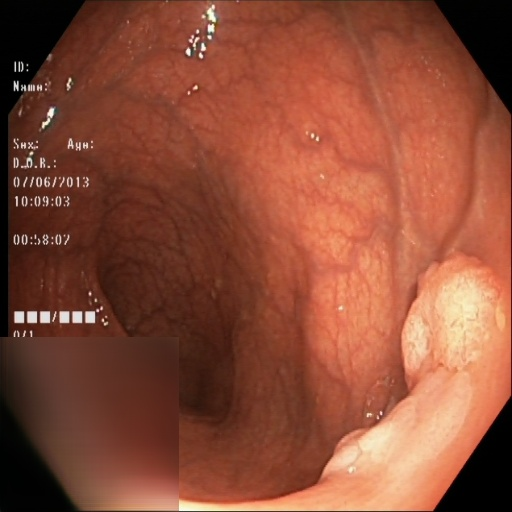
\includegraphics[width=\textwidth]{experiments/figures/nogreenframe.jpg}
         \caption{The same image as in Figure \ref{fig:GreenSquareOccluding} with the green square inpainted}
         \label{fig:GreenSquareOccludingFIX}
     \end{subfigure}
        \caption{Images where the troubling areas are removed before training}
        \label{fig:KvasirAnomaliesFIX}
\end{figure}


We propose three different types of inpainting to prove or disprove our two hypothesises.
\FloatBarrier
\subsection{Removing black corners}
The most straightforward experiment to conduct is to test how the removal of the black corners will affect the result.
As we propose in hypothesis \ref{hyp:a}, we believe that this masking can help with giving the classifier fewer areas with non-relevant information.
Figure \ref{fig:CornerMask} shows the mask used to inpaint the corners.

As we recall from section \ref{cha:endocolo}, the black edges around the images in our datasets is also, in general, present in medical colonoscopy images. By removing the black corners around the image, we do not change \textit{Kvasir specific} artefacts, but according to our first hypothesis, we believe we will get a higher classification accuracy since this removes areas with sparse information.

When classifying images during the testing stage, we need to take inpainting during training into account. 
\begin{enumerate}
\item We can do the same masking and inpainting on the test set. 
\item We can crop the image in a way that removes the black corners without inpainting.
\item We can forgo modifying the test data and just run the test set as is. 
\end{enumerate}


\paragraph{Method 1}
We tested method 1) in our paper ``Using preprocessing as a tool in medical image detection''~\cite{26254}.
The goal of this paper was related to hypothesis \ref{hyp:a} with the fact that we wanted to see how removing areas with sparse information affected the result of classification when training and testing on similar datasets. 
In the experiments run within this paper, both the training set and test set were inpainted. 
Since the focus of this task was to classify a test set we had from beforehand correctly, we had the option to preprocess the test set in addition to the training set without any penalties based on time restrictions. 
Our paper inpainted the test set as proposed in method 1) and from the results, it showed minimal improvement. The lack of improvement is mainly not connected to the fact that we inpainted the test set, but the fact that the test set came from the same distribution as the training set, and subsequently ended up with a model that overfitted to the data.
Given that we, in the end, want to classify images from a live colonoscopy, we have decided to forgo the inpainting of the test set using method 1).
By not augmenting the test set the experiments are also suited to reflect a larger research area of machine learning.



\paragraph{Method 2}
Method number 2) was the proposal of cropping the images during evaluation.  Thambawita et al. did similar methods in the Mediaeval 2018 conference but also had the same cropping during training. In the paper ``The Medico-Task 2018: Disease Detection in the Gastrointestinal Tract using Global Features and Deep Learning''~\cite{26205} we can see that this method worked with great success. 
The operation of just cropping images is also multiple times as fast as inpainting images, so it is feasible for a live recording.  
The downside of cropping the images from the test set is the fact that we do not have control over what we remove from the data. Given that the test set might come from a completely different distribution, we might unwillingly remove information we desire to keep. We do also run into the problem that cropping the images are not feasible when the sparse areas are within the image, and not at the outer edges.

\paragraph{Method 3}
The last proposed method is not to augment the images during testing. This method, since we are not preprocessing the test data at all, is the fastest when it comes to live classification. Without the augmentation, we risk getting a lower classification score, but we do not remove any data. Also, we make our results better reflect on how it will work on non-medical datasets.


In this thesis we will use method number 3). 
We base this decision on that we want the final product to have the option to be used live and be easily adaptable to other datasets.



%w
\subsection{Removing green squares}
The next major area in question is the removal of the green squares located in the bottom left area of some of the medical images.  This area is a Kvasir specific artefact and is found in 38\% of the images spanning five out of eight classes. 
By inpainting the lower left area we can see if our hypothesis \ref{hyp:b} is correct since here we are removing a dataset-specific feature that the network can use to determine classes. 
We have also chosen to inpaint every image, regardless of the green square is there or not. We do this so that the network can not ``learn'' that the pattern from the inpainted area correlates with the five classes with the green square, and hence defeating the purpose of the inpainting. Figure \ref{fig:GreenMask} shows the mask used to inpaint the lower left corner.

When classifying images during the testing stage, we have the same decision to take when it comes to inpainting of the test set.
\begin{enumerate}
\item We can either do the same masking and inpainting on the test set. 
\item We can crop the image in a way that removes the dataset-specific artefacts.
\item We can forgo modifying the test data and just run the test set as is. 
\end{enumerate}

To keep the consistency between to different inpainting methods, we use method 3) for the test set.
As with the black corners to be inpainted, we choose not to preprocess the test data, as this takes time, and should in theory not be necessary to get the right classification.
 

\subsection{Removing both corners and the green square}
The last set we want to test is the combination of both inpainting the green square and the black corner as shown with the mask in Figure \ref{fig:BothMask}. 
Here we hope that a combination of hypothesis \ref{hyp:a} and \ref{hyp:b} will give the strength of both methods without any harmful interference. 


\subsection{The generative modelling algorithms}
With the three masks discussed, we now want to present the generative modelling algorithms.
As addressed in section \ref{cha:BEW} our goal is to make new datasets without the unwanted artefacts based on the original dataset. 
We have chosen to use the two generative models presented in section \ref{cha:Explaining_autoencoders} and in section \ref{cha:Explaining_GANS}, namely Autoencoders and GANs.


As we recall from section \ref{cha:Explaining_autoencoders} the autoencoder and GAN\footnote{It is necessary to mention that regular GANs does not use a ground truth when training, though our modified GAN do.} networks both use a ground truth when training.
When training we need images that are already inpainted as a reference point. We solve this by zooming in the images to the limit that the edges are gone, as shown in figure \ref{fig:CornerMask}. When removing the dataset-specific features, we have the luxury that not all images contain the green square, giving us ample data for training after the images are sorted.
By removing the corners by zooming and by using images without artefacts during training, we have images where we know the whole ground truth, giving us the option to use MSE for backpropagation.


When training the GAN, we often do not need a ground truth behind the mask, as the network only tries to discern if the image is real or fake. This gives us in practice the same restrictions as with backpropagating with MSE.

\subsection{summary}
We have now talked about the three main masks we use, combined with the two generative models that make the datasets.
In total, we end up with six generated datasets, two for each mask type, and one unaugmented base case.

\textit{\textbf{Do i here talk about everything i didnt do?\\
\begin{itemize}
\item removing text, and the permutations regarding this
\item using a pixel CNN to inpaint
\item using the contextencoder as shown in first paper.
\end{itemize}
}}

\begin{figure}
     \centering
     \begin{subfigure}[t]{0.4\textwidth}
         \centering
         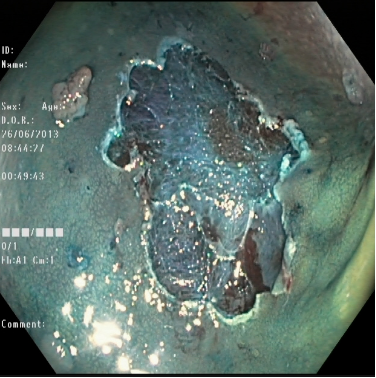
\includegraphics[width=\textwidth]{methodology/figures/nomask.png}
         \caption{Image from the original non-augmented dataset}
         \label{fig:CornerMask}
     \end{subfigure}
     \hfill
     \begin{subfigure}[t]{0.4\textwidth}
         \centering
         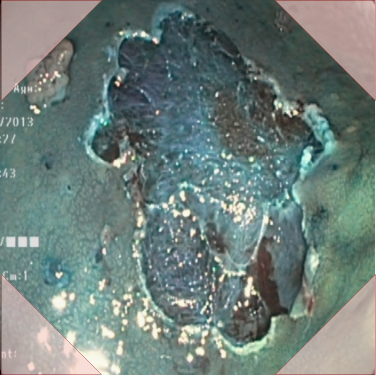
\includegraphics[width=\textwidth]{methodology/figures/cornermask.png}
         \caption{Red area shows the area masked in the first of the generated datasets}
         \label{fig:CornerMask}
     \end{subfigure}
     \hfill
     \begin{subfigure}[t]{0.4\textwidth}
         \centering
         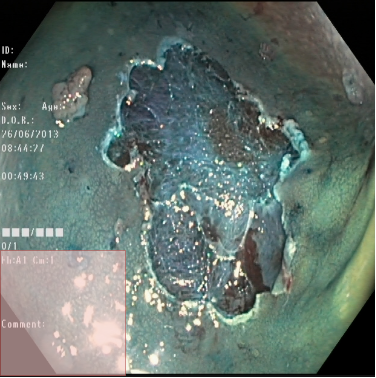
\includegraphics[width=\textwidth]{methodology/figures/greenmask.png}
         \caption{Red area shows the area masked by the second of the datasets}
         \label{fig:GreenMask}
     \end{subfigure}     
     \hfill
     \begin{subfigure}[t]{0.4\textwidth}
         \centering
         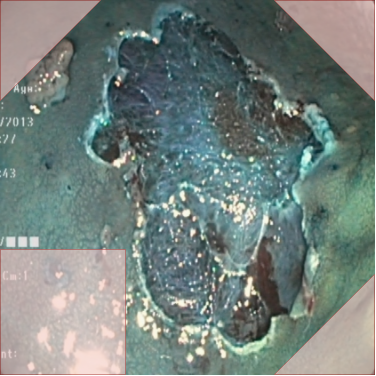
\includegraphics[width=\textwidth]{methodology/figures/bothmask.png}
         \caption{Red area shows the area masked by the third of the datasets}
         \label{fig:BothMask}
     \end{subfigure}
     \caption{All three mask types used in this thesis, and associated images used during training. At dataset in}
     \label{fig:masks}
\end{figure}



\FloatBarrier
\section{Design of the transfer learning experiments}
\label{cha:classifier}
To test the hypothesises we need a system in place to compare the datasets we generate with inpainting. As we recall, both our hypothesis is based on an improvement on a base score. 
To see if we have any improvement we propose to use a classifier based on transfer learning to see how the newly generated datasets gives a better classification score compared to the base dataset without augmentations.

We want to test our system with a range of different models and classifiers to test the validity of the system, and to make sure that our results are not just good out-layers.

Figure \ref{fig:KTLmodel} shows the general structure of the transfer learning model we use in this thesis. 


Hyperparameter optimisation of the models is a challenging task~\cite{runeMedico2018}. In this thesis, we have chosen to use automatic hyperparameter optimisation provided by SAGA~\todo{cite saga} to give us the optimal model for training. Based on our dataset, the optimal network was DenseNet121~\cite{DBLP:journals/corr/HuangLW16a} as our primary model for evaluation. 
In addition to an optimal model, we have chosen to use InceptionResNetV2~\cite{DBLP:journals/corr/SzegedyIV16} as a more general model. InceptionResNetV2 showed the highest top 1 and top 5 accuracies on imagenet when we designed the transfer learning program.

At the time of this writing, we have newer, more accurate models for imagenet. \todo{19 aug when i starded, IRV2 was the best model.}





\begin{figure}[h]
        \centering
        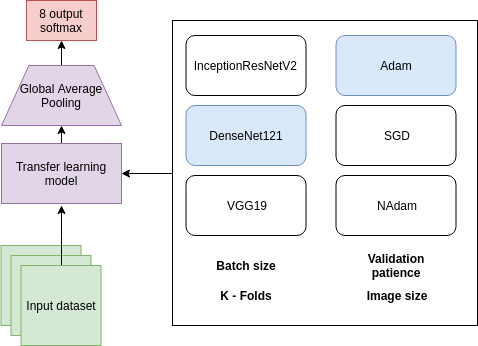
\includegraphics[scale=0.5]{methodology/figures/model.png}
        \caption{ The model we use for classifying with the most important options for the learning process. }
    \label{fig:KTLmodel}
\end{figure}


\subsection{models}
Here we go in depth in to how DN and IRV2 works.
\paragraph{Densenet}
\textit{\textbf{OMG I NEED TO WRIST STUFF HERE TOOOOOOOOOOOOOOOOOOO}}

\paragraph{Inception Residual Network architecture }
We can often see performance gains in our network architectures when we increase the size of the network. To increase the size, we can either increase the depth of the network, i.e. the number of layers, or we can increase the width of the network, i.e. increase the number of units per layer. Both methods are often easy to implement, but it often comes with the drawback of either increasing the number of parameters to train, which can result in overfitting, or it can result in the computation time of the network to increase to an unfeasible length.
To find a balance between accuracy and memory is often a hard task when it comes to not only medical images but images in general.

Szegedy et al. presented an architecture for the imagenet challenge with the intention of reducing the computational cost of training large neural networks by decreasing the number of parameters~\cite{DBLP:journals/corr/SzegedyLJSRAEVR14}. 
The network presented, GoogLeNet, used inception modules to reduce the computational cost.  Inception modules (networks within networks) tries to answer the question of witch convolution is the correct for each layer. Often it is up to the network architect to decide this, but with inception modules, the network chooses for itself.
In the GoogLeNet paper, the inception modules are the same as in Figure \ref{fig:Inception}, showing the option between $1 \times 1$, $3 \times 3$, $5 \times 5$ convolutions, and $3 \times 3$ max pooling, followed by a concatenation of the four options. \todo{do i mention the 1x1 that reduces dimentionality?}

Microsoft proposed another solution to training very deep neural networks in the form of residual modules~\cite{DBLP:journals/corr/HeZRS15} as shown in Figure \ref{fig:Residual}.
When using sufficiently large enough networks the backpropagation often encounter the problem with vanishing gradients. By adding a direct link between the layers, we counteract the vanishing gradient problem. A consequence we encounter when using residual modules is that instead of recreating the input for each layer, each layer learns only to modify the input value instead of completely recreating it.


\begin{figure}
     \centering
     \begin{subfigure}[t]{0.4\textwidth}
         \centering
         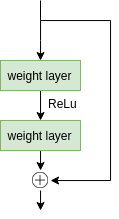
\includegraphics[width=0.5\textwidth]{methodology/figures/residual.png}
         \caption{Residual module concept as proposed in~\cite{DBLP:journals/corr/HeZRS15}}
         \label{fig:Residual}
     \end{subfigure}
     \hfill
     \begin{subfigure}[t]{0.55\textwidth}
         \centering
         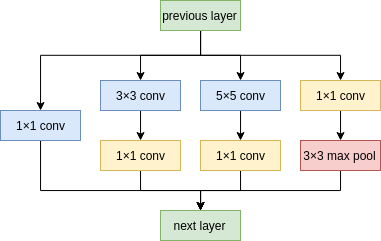
\includegraphics[width=\textwidth]{methodology/figures/inception.png}
         \caption{Inception module concept as proposed in~\cite{DBLP:journals/corr/SzegedyLJSRAEVR14}}
         \label{fig:Inception}
     \end{subfigure}
     \caption{The two main components in InceptionResNetV2}
     \label{fig:IRV2modules}
\end{figure}


Finally, combining the inception and residual modules, we end up with the modules used in InceptionResNetV2. \todo{more on this}


\subsection{pooling}
Write short about the pooling, maybe \todo{MICHAEL OR PAAL: \\do i bother talking about pooling?}
\paragraph{Global Average pooling}

\paragraph{Global max pooling }

\paragraph{No pooling}

\subsection{What does the different combination do to the result in our opinion (renamed to something cool sunglassemoji )}
Here we talk more bout what we believe the modules do to the result.

\subsection{summary}
We have in this section gone in-depth in to the transfer learning network.









\section{Libraries} 
With the general structure of the algorithms discussed, we will now go more in-depth in to the libraries used in the creation of the programs.

In this section, we will discuss the foundation of our code, important external libraries, and the setup and execution of our project.  
We first discuss the programming language in question, give insight into the reasoning behind it. Then we will look into the framework used for machine learning, and in detail how it implemented in our programming language. Lastly, we look into the wrapper we use to get a higher level of abstraction over our code, together with custom wrapper functions that are used by our wrapper. 

\subsection{Python}
When doing machine learning, the most popular languages, in no particular order, are Python, Java, R, C++, and C \todo{cite}. Some of these languages, like C and C++, are chosen for their speed, which is often a significant factor in Machine learning. Other languages, like R, is chosen because of its integration into the scientific community long before machine learning became a trend. The last group, consisting of Java and Python has gained popularity because of its already big user base and user-friendliness. Python is also the winner when it comes to machine learning because of, like R, its integration into the scientific community. 
Right now Python is the leading language for machine learning. Driven by this, there is considerable focus into making it faster, to compete with already fast languages, like the C family. 

Python is an interpreted, high-level, general-purpose programming language created in 1991.   It, like many other modern languages, is object-oriented and supports functional programming. 

Mainly because of the excellent support when it comes to machine learning, and the general "easy to use and no compiling" we have chosen python as the base for our code in this thesis. 



\subsection{Tensorflow}
Arguably the biggest reason for the success of machine learning in python lies in Tensorflow.\todo{cite} Tensorflow is a machine learning package developed by Google in \todo{year} and has since then become the leading framework for machine learning worldwide \todo{cote}.  
Tensorflow is in use by companies like AMD, Nvidia, eBay and Snapchat. 


\todo{something about projects with python, and how may uses}

Tensorflow is today a multi-language tool, but it had its origin in python. It is just in later years that other languages have gotten tensorflow support.  
The data flows through a graph network, where the objects in the graph describe the mathematical operations used in the machine learning, and the edges between graphs are the multidimensional arrays storing the weights associated with the operation in question. The name Tensorflow is a combination of the flow we experience during calculation and the tensors between the mathematical operations. 

As stated, Python, and subsequently machine learning in Python, would be much slower than a counterpart in C. Because of this, Tensorflow works as a layer of abstraction to code running in the C language. 
 
\todo{cpu vs gpu}
\todo{, CNTK, or Theano}



\subsection{Keras}
One of the least attractive things with tensorflow is its unnecessary complexity.  Even though Tensorflow offers more abstraction compared to running the code in pure C, the Tensorflow library can be unnecessarily complex.
As a result of this, many external libraries try to simplify many of the complexities that accompany tensorflow. 
Libraries like TFlearn was made as a modular and transparent deep learning library on top of tensorflow. It gives a higher-level API to Tensoflow to reduce complexity and speed up experiments. \todo{cite TFLEARN}
The most successful library for on top of Tensorflow is Keras \todo{cite keras}. 
Just as TFlearn, Keras is a high-level package written in python. It is capable of running on top of TensorFlow, CNTK, or Theano, which is the tree most popular machine learning libraries at this time. 
From their website they state that their four goals when creating Kears were:
\textbf{User friendliness. }\\
\textbf{Modularity. }\\
\textbf{Easy extensibility.}\\ 
\textbf{Work with Python. }\\

One of the core elements of Keras that makes it a better choice than just running, for instance, Tensorflow, is the concept of a model. A model in Keras is a way to organise the layers of the network in a more organised way, giving a better understanding of how the network is set up, and how each layer type contributes to the graph. \todo{more}

This thesis relies on Keras as a wrapper for tensorflow. As stated, the use of models and the simplicity of the language makes it an excellent choice of such a large project. Also, Keras has good support for convolutional operations which is the most used methods when managing images. Keras also has the most popular pretrained convolutional neural network models available in its package. \textit{Since one of our primary goal is to see how well our datasets generalise to the real world, transfer-learning will be a great tool to forgo unnecessary training}





    
\section{Custom functions for Keras, tensorflow and python}
\subsection{CWFC layer}
A problem often encountered when working with autoencoders which are not undercomplete is the fact that they learn to represent the data flawlessly. \cite{OvercompleteAE} 
When this problem arises, the network does not learn the fundamental features that define the dataset and instead passes the signal through the network without any consideration of the input data.
This flaw will often defeat the purpose of the algorithm, so data scientists often put in safeguards, like undercompleteness or regulisers, to combat this lack of feature learning. 
This problem extends to other types of generator networks where there are not sufficient compression or regularisation in the layers of the network.
Even though this problem often is solved by compressing the network into a space that can not contain the information exactly, the network does not always learn the features that define the network. 

We propose a custom ``channel-wise fully-connected layer'' in Keras to help with the problem of correctly learning features. This layer is based on the work done by Pathak et al. in their paper on content encoders\cite{Pathak_2016}.

The channel wise fully connected layer is primarily used in the GAN to transfer information within each feature map, without using convolutions to do it. As we recall, fully connected layers are often not suitable because of the large size of the weight layer associated with it. This layer is essentially a fully connected layer with groups, where the goal is to propagate the information within each feature map.
Given the latent space of $n \times n$ with $m$ feature maps, by not connecting the feature maps together in the fully connected layer we achieve a parameter reduction from $m^2n^4$ to $mn^4$ (ignoring bias terms) \cite{Pathak_2016}

With the ``channel-wise fully-connected layer'' the network can learn features from the entirety of the image, and not just local regions as it would with just convolutions. 

Listing \ref{listing:CWDense} shows the source code used for the channel-wise fully-connected layer.

\begin{minipage}{\linewidth}
\begin{listing}
\lstinputlisting[language=python]{methodology/CWDense.py}
\caption{The channel-wise fully-connected layer source code}
\label{listing:CWDense}
\end{listing}
\end{minipage}

\subsection{Subpixel}
When working with the generative adversarial network, we wanted to achieve more realistic representations at a reasonable image size. 
Making large scale images in generative adversarial networks has been a challenge that has only recently been cracked~\cite{DBLP:journals/corr/DentonCSF15}~\cite{DBLP:journals/corr/abs-1809-11096}.
As an early measure to fix this problem, we experimented with the use of a Sub-pixel layer as presented by Shi et al.~\cite{DBLP:journals/corr/ShiCHTABRW16} to give a more realistic output compared to just a standard conv-tanh layer.

\begin{figure}
\centering
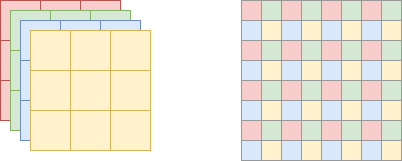
\includegraphics[scale=0.8]{methodology/figures/SubPixel.png}
\caption{How the layers in the sub pixel layer is stacked. Recreated from the SubPixel paper by Shi et al.~\cite{DBLP:journals/corr/ShiCHTABRW16}}
\label{fig:SubPixel}
\end{figure}






\subsection{Masklaod}
The most common way to load the dataset is to use the ML packs default ting.
I made my own thing to do this. i got cutting cropping graytone and rotating

\subsection{Self attention}
There are features in the images that are more important than others. One of the things we often want to preserve when we recreate images are hard edges. To get a semantically meaningful image,  we often want to differentiate between background and the mucosa. 
To see if the network can learn the features needed we are Introducing the Self Attention layer to help with this. 

\begin{minipage}{\linewidth}
\begin{listing}
\lstinputlisting[language=python]{methodology/SelfAttention.py}
\caption{The self attention layer source code}
\label{listing:Attention}
\end{listing}
\end{minipage}

\begin{figure}[h]
\centering
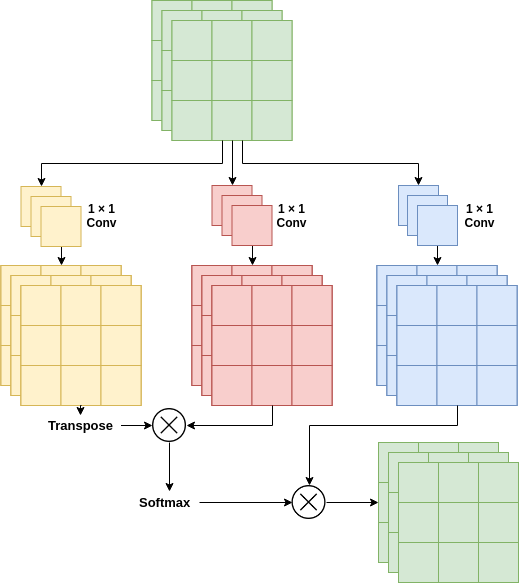
\includegraphics[scale=0.4]{methodology/figures/attention.png}
\caption{How the layers in the Self-Attention layer is stacked. Recreated from the Self-Attention  paper by Zhang et al.~\cite{DBLP:journals/corr/selfattention}}
\label{fig:Attention}
\end{figure}



\subsection{Masked loss}
A problem encountered for both the autoencoder and the GAN is what happens when the non-inpainted area gets too close to correct ground truth. 
As most of the image remains unchanged between the input-output space the loss for most of the image approaches 0 while the inpainted area stays at a high loss value for most of the training. 
As we recall from section \ref{cha:convNet}, we store our data as float32, and as the loss gets smaller and smaller, the squaring of the float32 gives at some point a number so small that the loss flips to a large integer and subsequently ruins the run. 

\todo{perhaps talk about the flip with image.}


To improve the stability we have modified the loss to only apply on the areas we inpaint, leaving the rest of the image withou a gradient to improve itself with.
Listing \ref{listing:maskedMSE} shows the source code for the masked MSE. 
For each point in the MSE we apply a binary mask, of the mask is zero, the point is not considered during backpropagation.


\begin{minipage}{\linewidth}
\begin{listing}
\lstinputlisting[language=python]{methodology/maskedMSE.py}
\caption{The self attention layer source code}
\label{listing:maskedMSE}
\end{listing}
\end{minipage}





\section{Stabilising the GAN}
Before we ended up with the model we used in the thesis we ran multiple experiments to make the generative adversarial network stable for training. 
In contrast to the autoencoder, the GAN does not use the ground truth as a reference point. Where the autoencoder always has a gradient based on the input data, the generator in the GAN gets its learning gradient from another network.

This lack of a ground truth gives the GAN many pitfalls that cause the training process to crash \footnote{Crashing is not the right word to use, but the result is the same: The learning process stops.}.


\paragraph{Normalise the inputs}
One of the first measures we did to prevent training collapse was to normalise the inputs. Instead of using images in the range 0 to 255 in pixel values we switched the values to  -1 to 1. 
Later, when the images were generated, we switched out the standard sigmoid output layer with a tanh output layer. As we wanted the output to be between -1 and 1, this was necessary, as the sigmoid only outputs between 0 and 1.

\paragraph{Using gaussian noise}
perhaps write about this



\paragraph{Normalising the batches}
One of the most significant challenges we encountered when training the adversarial network was the use of correct normalisation. 

The practice of training the discriminator with real and fake samples separately gave higher stability overall. 

The use of instance normalisation gave a better result compared to using batch normalisation. We believe this is contributed to the fact that the discriminator learned that the average pixel value was lower for the whole batch since the area inpainted had 0 as the pixel value.

The final model ended up not using batch or instance-normalisation. 



\paragraph{Avoiding sparse and vanishing gradients}
Most of the well-known networks use the ReLu\cite{Nair/2010/RLU/3104322.3104425} activation function \cite{DBLP:journals/corr/SimonyanZ14a} \cite{DBLP:journals/corr/SzegedyIV16} 
\cite{DBLP:journals/corr/HeZRS15}.
We saw the best result when we used non-sparse gradients during training. 
Instead of using ReLu we used the slightly modified LeakyReLu \cite{Maas2013RectifierNI}.

\todo{mention RReLu, but the number of parameters not worth it.}

In addition to trying to remove sparse gradients, we also wanted to address the problem with vanishing gradients during training. Given that we have fully saturated pixels (with the value of 1 or 255) and we have fully darkened pixels (with the value of -1 or 0) we, at the end of the experimentation phase, ended up removing the tanh layer. 
The removal of the tanh layer meant that the pixel values could be arbitrary on both positive and negative value, so we had to clip the value not to get an error at test time. 



\paragraph{Avoiding residual and inception layers}
When training the GAN experiments shows that the usage of both residual \cite{Rumelhart:1986:LIR:104279.104293} and inception \cite{DBLP:journals/corr/SzegedyLJSRAEVR14} models does note contribute to a good result when training the GAN.

Residual modules primary strength is that they always send the image/signal throughout the network in addition to the standard layers. Instead of the network needing to generate the whole image for each layer, the network instead adds or subtract from the original image for each layer.
This modification to the original image might seem reasonable when it comes to inpainting, but in reality, this does not work.  Given an image where we want to change only the inpainted area, the image is about 80\% unchanged. The network could focus on just filling in the inpainted area in theory, but in practice, the network tries to change the rest of the image in addition to the square. This incorrect inpainting gives us a generator that changes too much of the image and a discriminator that does not learn any important features since the input and output are relatively similar from the start.

Inception modules primary strength is the fact that the gradient can flow throughout the path most suited to the problem at hand.
We tested some training runs with inception modules, but the result was not impactful enough to continue to use this architecture.

From multiple training runs, it seems like just a straight forward encoder-decoder network for the generator yielded the best result. While the best result for the decoder was to use convolutions with stride do downsample the signal.

\todo{this might not be the right chapter for describing what layers are in the GAN, so please move}



\FloatBarrier
\section{Describe code}
We have, at this point, gone through the goal of our thesis, and shown how we want our result to be generated and evaluated in practice. 
We will now go more in-depth into the two networks used for generating the new datasets and go in-depth into the model we use for classification.


\subsection{autoencoder}
The autoencoder we used to generate the datasets used in this thesis bears a resemblance to the standard autoencoder proposed in chapter \ref{cha:Explaining_autoencoders}.

\paragraph{Loss, Optimiser}
To get the autoencoder to give the best result, we have chosen to use the mean square error loss as in equation~\ref{eq:MSE_form} and the Adam\cite{adam} optimiser.
The mean square error was a logical choice since we already have the ground truth and we only want to recreate the inpainted area based on what used to be there before the masking.
The Adam optimiser was chosen by the widespread usage in machine learning, coupled with the fact that it works well with sparse gradiens.

\paragraph{Encoder}
The input to the autoencoder were the masked images at $256 \times 256$px to compress the information in the encoder we imply used convolutions with a stride of 2. An option to using stride for the downsampling would be to use pooling, as described in section \ref{cha:pool}. Here, there are still room for experimentation.



\paragraph{Decoder}
between the encoder and decoder we added a 25\% dropout layer. This layer is the only reguliser in the network, though since the job were to inpaint and not recreate, the autoencoder needed information about a rather large area of the image, and hence had little possibility to overfit.

Upsampling could either be achieved with upconvolution or with upsampling.
Using upconvolution gives the network more variables (as the filters use weights, and upsampling does not), and hence would require more training. 

In this thesis we achieved the greatest results by using upsampling compared to upconvolution, though we can not rule out that upsampling would be better with more complex images, or at larger image sizes.

\vspace{5px}

To describe the model we will look at the example where we try to inpaint the green square in the image, and nothing else.

To train the autoencoder for inpainting, we divide the dataset in two, first images with the green square and images without the green square. We discard the images with the green square since they are not viable for training. 
The resulting dataset will only contain images without green sources.

\begin{figure*}[]
\centering
\begin{subfigure}[b]{0.45\textwidth}
    \centering
    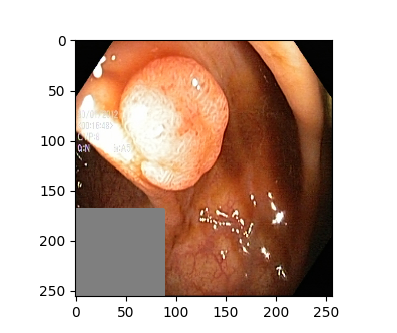
\includegraphics[width=\textwidth]{methodology/figures/masked_img.png}
    \caption{Image the autoencoder receives as an input }    
    \label{fig:AErec}
\end{subfigure}
\hfill
\begin{subfigure}[b]{0.49\textwidth}  
    \centering 
    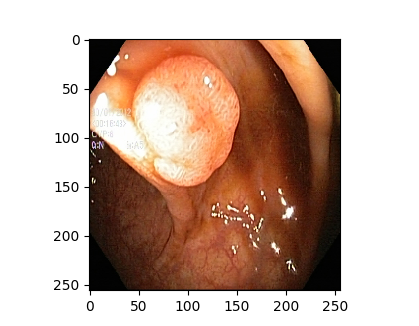
\includegraphics[width=\textwidth]{methodology/figures/whole_img.png}
    \caption[Hate to be this guy]%
    {{\small The missing part the autoencoder tries to replicate}}    
    \label{fig:AErep}
\end{subfigure}
\caption{A standard image taken in by the autoencoder} 
\label{fig:AEmasks}
\end{figure*}

The next step before training is to cut the images according to the mask provided. Figure \ref{fig:AErec} shows what the finished masking looks like, and \ref{fig:AErep} shows what we want to achieve after training.

We feed \ref{fig:AErep} into the autoencoder consisting of convolutional layers, leakyReLu layers, and a tanh layer.
\todo{more}
\todo{remember to talk about loss}


\subsection{Generative adversarial network}
The gan used the same generator discriminator elements as the Goodfellow gan, however the most significant difference is the fact that our model does not generate the image from Gaussian noise.

Instead of the standard Gaussian noise as input to the generator, the inpainted image is taken as input. Here, as in the autoencoder, we use stride to downsample the image. 


\todo{perhaps draw the shape?}



\subsection{Transfer learning classifier}
The dataset we are making with our generators needs to be classified. 

The classifier we use is based on the idea of reusing networks we already know apply well to the real world.
We have made a classifier that, by default, use one of the pretrained networks provided by the Keras framework.

\begin{table}[h]
\begin{center}
\small
\begin{tabular}{llllll}
\toprule
\multicolumn{1}{c}
{Model}             & Size   & Top-1 Accuracy & Top-5 Acc & Parameters  & Depth \\
\midrule
Xception          & 88 MB  & 0.790          & 0.945          & 22,910,480  & 126   \\
VGG16             & 528 MB & 0.713          & 0.901          & 138,357,544 & 23    \\
VGG19             & 549 MB & 0.713          & 0.900          & 143,667,240 & 26    \\
ResNet50          & 98 MB  & 0.749          & 0.921          & 25,636,712  & -     \\
ResNet101         & 171 MB & 0.764          & 0.928          & 44,707,176  & -     \\
ResNet152         & 232 MB & 0.766          & 0.931          & 60,419,944  & -     \\
ResNet50V2        & 98 MB  & 0.760          & 0.930          & 25,613,800  & -     \\
ResNet101V2       & 171 MB & 0.772          & 0.938          & 44,675,560  & -     \\
ResNet152V2       & 232 MB & 0.780          & 0.942          & 60,380,648  & -     \\
ResNeXt50         & 96 MB  & 0.777          & 0.938          & 25,097,128  & -     \\
ResNeXt101        & 170 MB & 0.787          & 0.943          & 44,315,560  & -     \\
InceptionV3       & 92 MB  & 0.779          & 0.937          & 23,851,784  & 159   \\
InceptionResNetV2 & 215 MB & 0.803          & 0.953          & 55,873,736  & 572   \\
MobileNet         & 16 MB  & 0.704          & 0.895          & 4,253,864   & 88    \\
MobileNetV2       & 14 MB  & 0.713          & 0.901          & 3,538,984   & 88    \\
DenseNet121       & 33 MB  & 0.750          & 0.923          & 8,062,504   & 121   \\
DenseNet169       & 57 MB  & 0.762          & 0.932          & 14,307,880  & 169   \\
DenseNet201       & 80 MB  & 0.773          & 0.936          & 20,242,984  & 201   \\
NASNetMobile      & 23 MB  & 0.744          & 0.919          & 5,326,716   & -     \\
NASNetLarge       & 343 MB & 0.825          & 0.960          & 88,949,818  & -        \\   
\bottomrule
\end{tabular}
\end{center}
\caption{Models provided by keras}
\label{tab:Kaeras_app}
\end{table}

Table \ref{tab:Kaeras_app} shows the pretrained networks available to load in the Keras framework. 
When training we did some extra steps at the end, namely added global average pooling and a fully connected layer with the desired number of outputs (usually eight classes, and eight outputs)




\section{Describe project}
Here i am going to explain the projects\\
Here i am going to explain the projects\\
Here i am going to explain the projects\\
Here i am going to explain the projects\\
Here i am going to explain the projects\\
Here i am going to explain the projects\\
Here i am going to explain the projects\\
Here i am going to explain the projects\\
Here i am going to explain the projects\\
Here i am going to explain the projects\\
Here i am going to explain the projects\\

\section{Summary}
In this chapter we have, in more detail, looked at the process and purpose of inpainting and classifying.
We started with the discussion regarding where to inpaint, and the problem statements we wanted to test for each of the inpaintings. 
We made a decision regarding if inpainting of the test set were feasible, and decided the two types of generative modelling algorithms we use in this thesis. 
We looked at the need for a classification model to discern the results of our inpainting and decided to use transfer learning to represent a real-world scenario better.
We looked into the two transfer learning models we use in this thesis, namely Densenet121 and InceptionResNetV2, and gave a brief overview of their similarities and differences.

After a more conceptual view, we talked more about how we would achieve the experiments in practice.  Here we talked about why we chose python, tensorflow and keras, followed by custom functions needed for our machine learning algorithms. 
We ended the chapter with the description of the three models in practice.

 



%\chapter{Methods} \label{cap:methods}
%
  
  \subsection{Removing borders}
    A normal picture from the kvasir dataset, as seen earlier, has more to it than just the picture we are after.
    As mentioned over the less clutter we can get in our data the better. So one of the first thing we should do is to remove the frame.
    \begin{figure}[ht]
      \centering
      \begin{minipage}[b]{0.45\textwidth}
	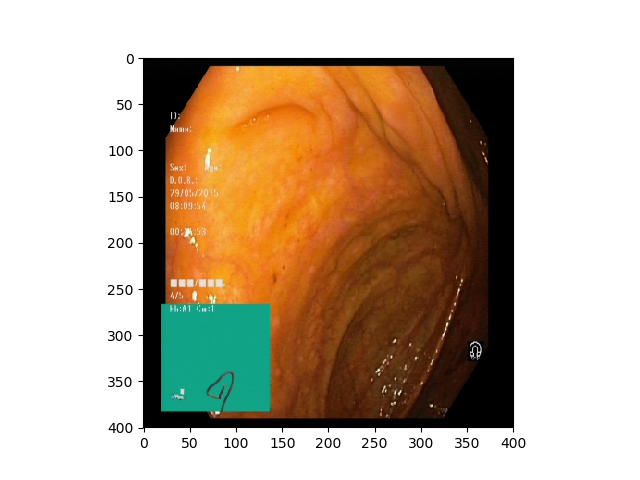
\includegraphics[width=\textwidth]{methods/figures/No_crop.png}
	\caption{Original image with no edges removed}
      \end{minipage}
      \hfill
      \begin{minipage}[b]{0.45\textwidth}
	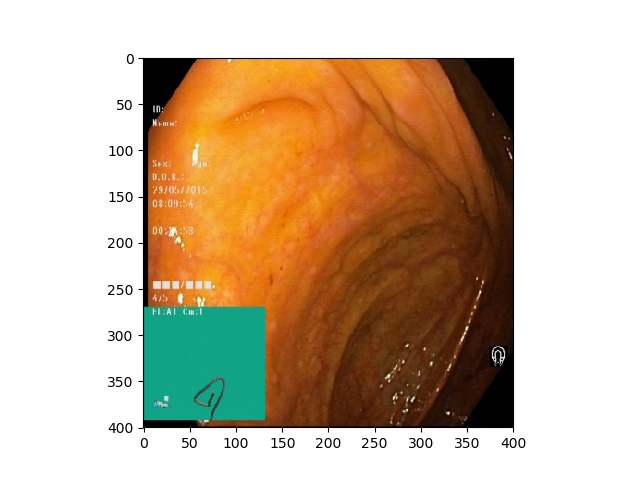
\includegraphics[width=\textwidth]{methods/figures/Crop.png}
	\caption{Edges of the image removed}
      \end{minipage}
    \end{figure}
    The biggest reason why this is done is because of the lack of information in the black, uniform pixels. Since the 
    black area differs in every image, the area is saved as a feature. This feature contains no relevant information for the analysis,
    so it is easier if it is just discarded. \\
    
    The image is cropped using 2 simple algorithms, first we run a morphological opening with a $5\times5$ kernel on a black/white copy of the image. 
    This will remove any unwanted artifacts and/or text in the black area. Now that the border is guarantied black, we can do a simple crop where the border stops.
    
    %identical
    %black beckomes a featire, with features 
    
  \subsection{Adjusting brightness and contrast}
  TODO LATER.
  
  \subsection{Removing artifacts and saturated spots}
  In addition to the border areas there are also other areas that bear little to no information. This is the bright spots where the light from the camera-pill is saturating the CCD in the pill.
  White areas like this can be treated as a feature, and as with the border, this feature contains no relevant information.
  %TODO cite Zeno Albisser
  In the article \textit{Computer-Aided Screening of Capsule Endoscopy Videos} from Zeno Albisser it is proposed a way to remove bright areas by using a horizontal gradient over the bright areas.
  In the loading of the images a similar treatment %TODO find word
  of the images is done.
  
  \subsection{Using a Contextencoder to predict image parts}
  At this point we have used naive methods to enhance the data. Another big part of the image has not been mentioned this far, and that is the green square many of the images contains.
  
  \begin{figure}[h]
    \centering
    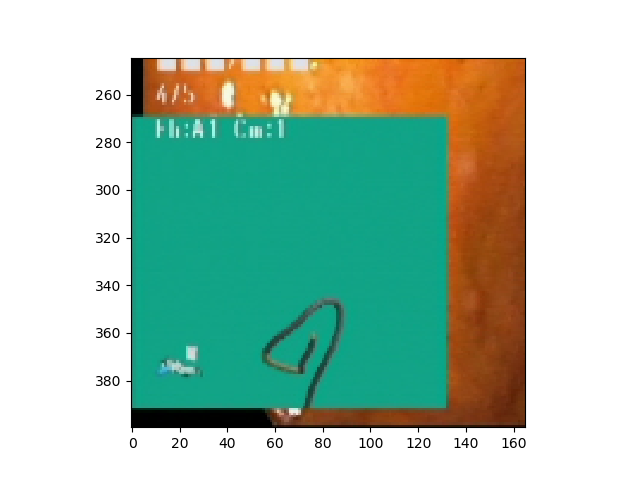
\includegraphics[scale=0.5]{methods/figures/Green_square.png}
    \caption{A typical example of a green square containing information about where in the GI-tract the image is taken from}
  \end{figure}
  
  A way to remove the square is to continue to use a naive method, perhaps with a horizontal gradient or a similar technique. 
  However we can use a convolutional neural net to try to predict what would be behind the area. 
  
  \subsubsection{Using a GAN}
  As described earlier in the thesis %TODO describe earlier
  we can use an adversarial network to generate images. 
  The general Contextencoder has three main parts: Encoder, decoder and a Discriminator.
  
  \begin{figure}[ht]
    \centering
    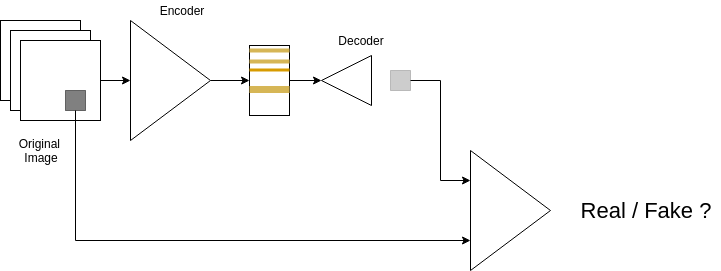
\includegraphics[scale=0.5]{methods/figures/Contextencoder.png}
    \caption{A simple Contextencoder}
  \end{figure}
  
  %TODO MENTION THAT WE ARE NOT TRAININ ON GREEN IMGS
  %TODO MENTION THAT WE ARE NOT TRAININ ON GREEN IMGS
  %TODO MENTION THAT WE ARE NOT TRAININ ON GREEN IMGS
  First an (often random) area is removed from the original image, and is stored as a copy. Then the decoder takes the reminding image and compresses it to a latent space. From there 
  the encoder tries to build a new image that is the same size as the missing peace. \\
  After the peace is made it is sent to the discriminator, together with the original peace. The discriminator takes both the generated image as well as the original image and tries to give a prediction if it
  believes if the part it got was a generated or original image.
  Training and evaluation is the same as described in the general description of how an generative adversarial network is working.
  
  \subsection{Using a Variational Autoencoder to train the adversarial network}
    This chapter talks about the use of a Variational autoencoder to train the generator.
    
    
    
  \subsubsection{Setup of the GAN}
  Using the Contextencoder described we made 3 %TODO make 2 more programs
  similar programs for image prediction.\\
  \vspace{5px}
  \textbf{Random masker:} The first program is designed to work with any data as long as you train the weights on sufficient data. The random masker trains on images where the area masked is 
  uniformly distributed throughout the images. This approach is highly general, and will give a better masking on nongreen squares, compared to the corner masker.  
  
  \vspace{5px}
  \textbf{Corner masker:} The corner masker is designed to only mask the bottom left corner where the green square is located, this means that it is better at finding the area behind the green square, but it is much 
  worse at predicting any other part of the image.
  
  \vspace{5px}
  \textbf{Categorical masker:} The categorical masker is a mix between the two prior models. The categorical masker divides the image in to 9 different equally placed squares, and only masks those areas. %TODO Is middle one removed?
  The result is a mix between a general approach and a specific corner approach.

  
  \subsubsection{Result of the GAN}
  The result of the trained weights can be found at %TODO adress
  It is part of a pygame demo, that can take any image and predict the area marked, based on the loaded weights.\\
  
  \vspace{5px}
  \textbf{Random masker:}
  %TODO images?
  As we can see from the images, the area is not perfectly masked, but these weights can be used on any part of the image with the same result.
  
  \vspace{5px}
  \textbf{Corner masker:}  
  %TODO images?
  This is the prediction given the weights trained only on the bottom left corner. This result gives a better prediction than the random masker, but can not be used other places in the image
  
  \vspace{5px}
  \textbf{Categorical masker:} 
  %TODO images?
  DONT KLNOW yet
  
  
  
  
  
  
  
\section{Making the dataset larger}
  One of the reasons why machine learning has become a hot topic the last years is the amount of data stored the last century. %TODO find rightt word
  

\chapter{Experiments} \label{cap:experiments}
\section{Datasets}
    \todo{write about the datasets show images}
    
    \subsection{CVC-356}
    \subsection{CVC-12k}
    \subsection{CVC-612}

\section{Metrics}
    \subsection{TP, TN, FP FN}
    \subsection{Precicion}
    \subsection{recall}
    \subsection{F1}
    \subsection{MCC}
    
\section{Setup of experiments}

\section{format of experiments}
    \subsection{Inpaint}
    \subsection{Classifying}
    
\section{Inpainting Kvasir}
    \subsection{Black corners}
    \subsection{Green square}
    \subsection{Text}
    \subsection{Combination}
    \subsection{Random masking}
    
\section{Kvasir -> CVC612}
\section{Kvasir -> CVC 12k}
\section{Kvasir -> CVC356}

\section{Summary
}



\chapter{Discussion and future work} \label{cap:future}
The task of making general models to cover a broad aspect of medical images is still a widely researched area today, and most likely, it will continue to be so in the future. There are a  plethora of different ways to build models for the medical domain, and in most of them, there is room for improvement.

\section{Conclusion}
We have seen the power of inpainting when it comes to datasets previously unseen during training. Both shown in our publications and the thesis, we have an increase in classification score on multiple types of inpainting.
Unfortunately, we get some inconsistencies results during testing, which means that we cannot recommend any method over another, as the result show that the type of inpainting is closely related to the dataset.
In general, we saw an improvement when it came to inpainting, but the improvement differed between the two datasets. 

For the CVC 356 dataset removing artefacts within the image gave the best result for both models. When inpainting areas within the image the GAN won five out of six times, making it the best model for inpainting  areas with great detail. The good results lie also in the network used. The Densenet model worked excellent for the classification of this dataset.


For the CVC 12k dataset, we saw lower scores in general, confirming that this dataset is notoriously harder to classify. We did get the only improvement using inpainting of the borders around the Kvasir dataset during training, giving us believe that the network gained accuracy from the ´´distilled'' data provided when the borders were removed. 

The Kvasir dataset did not see anything else than a marginal improvement to an already high score. We will not draw any conclusions from the result, given the statistical uncertainties when the scores are so close to the baseline.


Finally, the act of inpainting both the corners and the green square gave us the highest score on the CVC 356 dataset, and a decent score for the CVC 12k dataset. The excellent scores give us some merit to believe that the two inpainting models can work together without interfering destructively with each other. 

\vspace{5px}

We can recall \ref{hyp:a} regarding the removal of sparse information to help with image classification. From our tests, we conclude that this hypothesis is correct given the right dataset and model. 
In general, we saw a clear advantage of removing sparse regions. 

Hypothesis \ref{hyp:b} about the removal of dataset-specific artefacts we also conclude to be correct, given the right dataset and model. 
Based on our results we can see a clear difference between the inpainted images and the baseline. 
Using a dataset like CVC 356 gave us better result with almost every configuration when inpainting based on hypothesis \ref{hyp:b}

\vspace{5px}
\noindent \textit{1. Can the process of redrawing an area with a new more relevant information, of sparse areas in datasets help with training and classification performed by machine learning? If so, how detailed should the inpainting be?}\\

Repainting areas with sparse information help with classification, given that the test dataset does not have even bigger areas with sparse information compared to the training dataset. When it comes to the detail of inpainting, we do not draw any definite conclusions, but the results tend to show that a smother form if inpainting is better.




\vspace{5px}
\noindent \textit{2. Can inpainting of dataset-specific artefacts help with the classification of previously unseen data done by machine learning? If so, how detailed should the inpainting be?}

Repainting areas containing artefacts helps significantly with classification. With the right setup, we saw results both doubling and tripling the MCC score. The models show an advantage using the GAN for inpainting, giving us an indication that the more details, the better. 


In addition to the results presented in this thesis we have during the writing of this thesis published two articles to support our results.

\paragraph{Using prerocessing as a tool in medical image detection}
The first paper was presented at the ACM conference in Nice, France worked exclusively on the Kvasir dataset. The result we published showed a small increase in classification perfromance when inpainting sparse regions. 
Here we showed that even though we tested and trained on the same dataset, we saw performance gains.

\paragraph{Unsupervised preprocessing to improve generalisation for medical image classification}
The second paper presented at the ISMICT conference in Oslo, Norway expanded the work presented in the ACM conference in 2018.
The presented result used an average of multiple runs instead of K-fold cross-refenrence, though the same datasets and transfer learning models were used.
Here we saw similar results as the findings presented in this thesis. 





\todo{Her bør du gjenta seksjon 1.5. Få også med en mer detaljert diskusjon om HYPOTESENE holder og hva svaret er på SPØRSMÅLENE (med underspørsmål) fra seksjon 1.2. Her må du henvise tilbake til problemstillingen og vise at du har løst oppgaven du har spesifisert. Igjen si at resultater er publisert.}


\section{Future work}
The Work done in this thesis show that there might be improvements when classifying images with non-perfect information. There is still much work that can be done, both to improve inpainting and classification, and to better understand the ´´black box'' that is machine learning. 

\paragraph{Better performance GAN}
Since the start of this project, there have been published multiple new papers concerning making realistic GANs including \cite{DBLP:journals/corr/abs-1809-11096} \cite{DBLP:journals/corr/abs-1812-04948}. As this is still a relatively new research field, there are still many improvements that could be done to make the models better.
The best way to improve the GAN models is just to let them train longer. The latest model used to generate the inpainted dataset were running for approximately 40 hours, which is still away from reaching the best result. By using more time when training the models, we might achieve even better MCC when classifying the medical datasets.
Another way that might improve the GAN is better utilisation of the channel-wise fully-connected layer. In this thesis, this layer was a quintessential part of the result we got, and by tweaking the layers might give even better results.

\paragraph{Looking into using the generated images for classification}
The images generated by the GAN will most likely have features that are an essential part of the original image. If this is the same underlying features that are used in, for instance, DenseNet or Inceptionresnet we might not need to paste the inpainted area back into the original image.
Further research regarding the generator learning features from the different classes could show good results.
Another promising aspect of this is to let the discriminator guess the class in addition to real and fake images. If that is the case, the generator needs to learn features that define the different classes. We can see from images like Figure \ref{fig:p_GAN_BOTH2} that this, to a case, is already happening without making an auxiliary GAN.
In the end, the ability to compress the images with a GAN or AE might give us a new way to classify images.

\paragraph{Experiment with self attention}
We touched upon self attention in section \ref{cha:attention}. Though we did some experiments with self attention, more testing is required for a conclusion if its good or not in the context of this thesis. Future work should be to implement the attention layer into the GAN to see if the reconstructed areas can become better. 

5%\paragraph{Cropping of images}
%dsgfsgsgw

\paragraph{Make a generator for new data}
We have used the GAN and AE to exclusively inpaint images, but both models can, without any extensive modifications,  generate data from the same image domain from the original dataset, just like the original DCGAN ~\cite{DBLP:journals/corr/RadfordMC15} does.  
By using the dataset to generate new previously unseen data, we might help classification not to overfit.

\paragraph{Improving the program to work cross domain}
For future work, we would like to automate the process of inpainting by making the models look better, and give the user the option of choosing their areas to inpaint. The model presented can be used at any dataset, but the user has to edit the masks manually. 

\paragraph{Using OCR to remove text}
We tested the option to remove text using an Optical Character Recognition (OCR) during this thesis, but the time used by OCR algorithms are too slow to work in real-time. Combining the system presented in this thesis with a system like Rosetta~\cite{borisyuk2018rosetta} or EAST~\cite{DBLP:journals/corr/ZhouYWWZHL17} might give a speedup, but at the conclusion of this thesis, we are not able to run OCR and classification without a multi-GPU setup.


\paragraph{NASNetLarge}
When we chose our general model for classification back in August 2018, we used InceptionResNetV2 as our model. Since then F. Chollet has added NASNetLarge~\cite{DBLP:journals/corr/ZophVSL17} to the list of transfer learning models. NASNetLarge has a higher accuracy on the imagenet model and should possibly be the standard model for the classification.




%\section{How to view the result?}
  \subsection{The rate of success}
  What is a good result, how to measure?\\
  \textbf{FP,TN,FN,TP}\\


%\chapter{Conclusion} \label{cap:conclution}
%\input{conclusion/conclusion.tex}

%\chapter{Future Work} \label{cap:future}
%The task of making general models to cover a broad aspect of medical images is still a widely researched area today, and most likely, it will continue to be so in the future. There are a  plethora of different ways to build models for the medical domain, and in most of them, there is room for improvement.

\section{Conclusion}
We have seen the power of inpainting when it comes to datasets previously unseen during training. Both shown in our publications and the thesis, we have an increase in classification score on multiple types of inpainting.
Unfortunately, we get some inconsistencies results during testing, which means that we cannot recommend any method over another, as the result show that the type of inpainting is closely related to the dataset.
In general, we saw an improvement when it came to inpainting, but the improvement differed between the two datasets. 

For the CVC 356 dataset removing artefacts within the image gave the best result for both models. When inpainting areas within the image the GAN won five out of six times, making it the best model for inpainting  areas with great detail. The good results lie also in the network used. The Densenet model worked excellent for the classification of this dataset.


For the CVC 12k dataset, we saw lower scores in general, confirming that this dataset is notoriously harder to classify. We did get the only improvement using inpainting of the borders around the Kvasir dataset during training, giving us believe that the network gained accuracy from the ´´distilled'' data provided when the borders were removed. 

The Kvasir dataset did not see anything else than a marginal improvement to an already high score. We will not draw any conclusions from the result, given the statistical uncertainties when the scores are so close to the baseline.


Finally, the act of inpainting both the corners and the green square gave us the highest score on the CVC 356 dataset, and a decent score for the CVC 12k dataset. The excellent scores give us some merit to believe that the two inpainting models can work together without interfering destructively with each other. 

\vspace{5px}

We can recall \ref{hyp:a} regarding the removal of sparse information to help with image classification. From our tests, we conclude that this hypothesis is correct given the right dataset and model. 
In general, we saw a clear advantage of removing sparse regions. 

Hypothesis \ref{hyp:b} about the removal of dataset-specific artefacts we also conclude to be correct, given the right dataset and model. 
Based on our results we can see a clear difference between the inpainted images and the baseline. 
Using a dataset like CVC 356 gave us better result with almost every configuration when inpainting based on hypothesis \ref{hyp:b}

\vspace{5px}
\noindent \textit{1. Can the process of redrawing an area with a new more relevant information, of sparse areas in datasets help with training and classification performed by machine learning? If so, how detailed should the inpainting be?}\\

Repainting areas with sparse information help with classification, given that the test dataset does not have even bigger areas with sparse information compared to the training dataset. When it comes to the detail of inpainting, we do not draw any definite conclusions, but the results tend to show that a smother form if inpainting is better.




\vspace{5px}
\noindent \textit{2. Can inpainting of dataset-specific artefacts help with the classification of previously unseen data done by machine learning? If so, how detailed should the inpainting be?}

Repainting areas containing artefacts helps significantly with classification. With the right setup, we saw results both doubling and tripling the MCC score. The models show an advantage using the GAN for inpainting, giving us an indication that the more details, the better. 


In addition to the results presented in this thesis we have during the writing of this thesis published two articles to support our results.

\paragraph{Using prerocessing as a tool in medical image detection}
The first paper was presented at the ACM conference in Nice, France worked exclusively on the Kvasir dataset. The result we published showed a small increase in classification perfromance when inpainting sparse regions. 
Here we showed that even though we tested and trained on the same dataset, we saw performance gains.

\paragraph{Unsupervised preprocessing to improve generalisation for medical image classification}
The second paper presented at the ISMICT conference in Oslo, Norway expanded the work presented in the ACM conference in 2018.
The presented result used an average of multiple runs instead of K-fold cross-refenrence, though the same datasets and transfer learning models were used.
Here we saw similar results as the findings presented in this thesis. 





\todo{Her bør du gjenta seksjon 1.5. Få også med en mer detaljert diskusjon om HYPOTESENE holder og hva svaret er på SPØRSMÅLENE (med underspørsmål) fra seksjon 1.2. Her må du henvise tilbake til problemstillingen og vise at du har løst oppgaven du har spesifisert. Igjen si at resultater er publisert.}


\section{Future work}
The Work done in this thesis show that there might be improvements when classifying images with non-perfect information. There is still much work that can be done, both to improve inpainting and classification, and to better understand the ´´black box'' that is machine learning. 

\paragraph{Better performance GAN}
Since the start of this project, there have been published multiple new papers concerning making realistic GANs including \cite{DBLP:journals/corr/abs-1809-11096} \cite{DBLP:journals/corr/abs-1812-04948}. As this is still a relatively new research field, there are still many improvements that could be done to make the models better.
The best way to improve the GAN models is just to let them train longer. The latest model used to generate the inpainted dataset were running for approximately 40 hours, which is still away from reaching the best result. By using more time when training the models, we might achieve even better MCC when classifying the medical datasets.
Another way that might improve the GAN is better utilisation of the channel-wise fully-connected layer. In this thesis, this layer was a quintessential part of the result we got, and by tweaking the layers might give even better results.

\paragraph{Looking into using the generated images for classification}
The images generated by the GAN will most likely have features that are an essential part of the original image. If this is the same underlying features that are used in, for instance, DenseNet or Inceptionresnet we might not need to paste the inpainted area back into the original image.
Further research regarding the generator learning features from the different classes could show good results.
Another promising aspect of this is to let the discriminator guess the class in addition to real and fake images. If that is the case, the generator needs to learn features that define the different classes. We can see from images like Figure \ref{fig:p_GAN_BOTH2} that this, to a case, is already happening without making an auxiliary GAN.
In the end, the ability to compress the images with a GAN or AE might give us a new way to classify images.

\paragraph{Experiment with self attention}
We touched upon self attention in section \ref{cha:attention}. Though we did some experiments with self attention, more testing is required for a conclusion if its good or not in the context of this thesis. Future work should be to implement the attention layer into the GAN to see if the reconstructed areas can become better. 

5%\paragraph{Cropping of images}
%dsgfsgsgw

\paragraph{Make a generator for new data}
We have used the GAN and AE to exclusively inpaint images, but both models can, without any extensive modifications,  generate data from the same image domain from the original dataset, just like the original DCGAN ~\cite{DBLP:journals/corr/RadfordMC15} does.  
By using the dataset to generate new previously unseen data, we might help classification not to overfit.

\paragraph{Improving the program to work cross domain}
For future work, we would like to automate the process of inpainting by making the models look better, and give the user the option of choosing their areas to inpaint. The model presented can be used at any dataset, but the user has to edit the masks manually. 

\paragraph{Using OCR to remove text}
We tested the option to remove text using an Optical Character Recognition (OCR) during this thesis, but the time used by OCR algorithms are too slow to work in real-time. Combining the system presented in this thesis with a system like Rosetta~\cite{borisyuk2018rosetta} or EAST~\cite{DBLP:journals/corr/ZhouYWWZHL17} might give a speedup, but at the conclusion of this thesis, we are not able to run OCR and classification without a multi-GPU setup.


\paragraph{NASNetLarge}
When we chose our general model for classification back in August 2018, we used InceptionResNetV2 as our model. Since then F. Chollet has added NASNetLarge~\cite{DBLP:journals/corr/ZophVSL17} to the list of transfer learning models. NASNetLarge has a higher accuracy on the imagenet model and should possibly be the standard model for the classification.






\backmatter{}
\printbibliography



\chapter{Appendix}
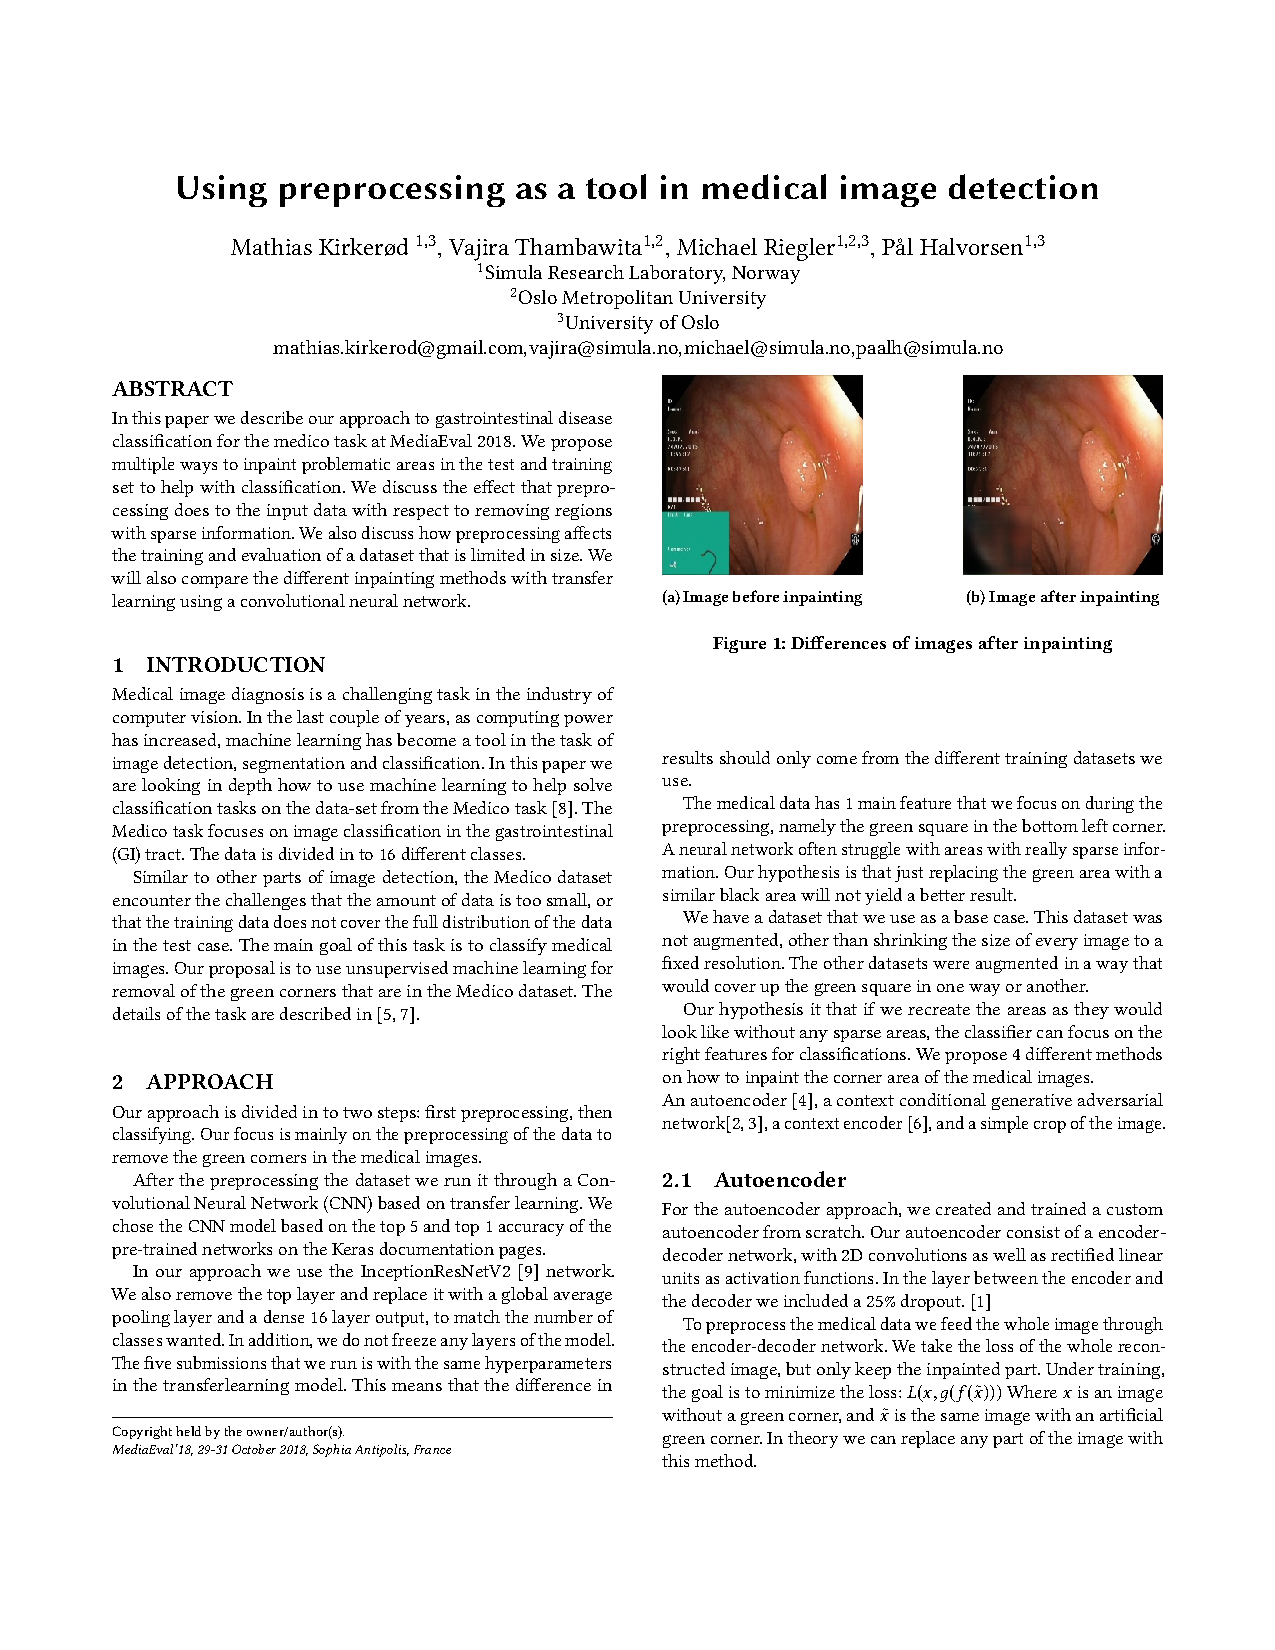
\includepdf[pages={1-3}]{appendix/PaperMediaEval.pdf}
\includepdf[pages={1-6}]{appendix/PaPerIEEE.pdf}
%\begin{appendices}
%\chapter{The preparation Process} \label{ap}
%\input{preparation.tex}
%\end{appendices}

\end{document}
